\documentclass{article}

% Working manuscript entry point for the NeurIPS 2026 Evaluations & Datasets paper.
% Keep the stock template file `neurips_2026.tex` unchanged for reference.

\usepackage[eandd]{neurips_2026}

\usepackage[utf8]{inputenc}
\usepackage[T1]{fontenc}
\usepackage{hyperref}
\usepackage{url}
\usepackage{booktabs}
\usepackage{amsfonts}
\usepackage{amsmath}
\usepackage{amssymb}
\usepackage{nicefrac}
\usepackage{microtype}
\usepackage{xcolor}
\usepackage{graphicx}

\title{JaxARC: A JAX-native environment for reinforcement learning and adaptation on ARC}

\author{Anonymous Authors}

\begin{document}

\maketitle

\begin{abstract}
% Abstract recipe:
% 1. Set up the scientific problem: ARC as an RL domain.
% 2. State the gap: CPU-bound environments bottleneck research; no multi-algorithm baselines exist.
% 3. State the contribution: JaxARC + throughput + baseline benchmark.
% 4. State the main empirical findings: algorithm ordering, task-family variation, observation analysis.
% 5. State the implication: practical substrate for future ARC RL research.
%
% Keep to one paragraph. Avoid: solve, breakthrough, state of the art, robust transfer.

The Abstraction and Reasoning Corpus (ARC) poses a distinctive challenge for reinforcement learning: agents must learn to edit grids through sequential actions, guided only by sparse rewards, across hundreds of structurally diverse tasks. Studying RL on ARC at scale has been impractical because existing environments run on the CPU and cap throughput at roughly 60,000 steps per second. We introduce JaxARC, an open-source, JAX-native ARC environment that runs entirely on hardware accelerators, reaching over 100 million steps per second on a single H100 GPU---a $5{,}400\times$ speedup over the prior ARCLE environment at matched batch sizes. To demonstrate what this throughput enables, we provide three contributions beyond the environment itself. First, we profile the computational overhead of different observation and action wrappers, showing that answer-visible configurations substantially improve learnability while richer observation channels carry measurable throughput costs. Second, we present the first multi-algorithm RL baseline benchmark for ARC, evaluating PPO, DQN, PQN, and REINFORCE across six ARC-AGI difficulty tiers and six ConceptARC concept groups, with five seeds and 10 million steps per condition. The results reveal a consistent algorithm hierarchy---PPO dominates, followed by REINFORCE, with DQN and PQN trailing---and large performance variation across task families, from near-perfect returns on ConceptARC Count to negligible progress on ARC-AGI Hard. JaxARC, together with these baselines and analyses, provides a practical foundation for systematic RL research on abstract reasoning.
\end{abstract}

\section{Introduction}
% Purpose:
% Frame the paper as an ED-track contribution, not a systems or solver paper.
%
% Must do:
% - Introduce ARC as a benchmark increasingly studied through test-time adaptation and compute.
% - Explain why systematic support-to-query evaluation is hard without a practical executable substrate.
% - Introduce JaxARC as the enabler of that evaluation.
% - Preview the central empirical finding: support-side gains do not become hidden-query success.
% - End with a crisp contributions list.
%
% Keep out:
% - Long API or implementation detail.
% - Overstated speed bragging.
% - Any implication that the baselines solve hidden queries.
%
% Primary sources:
% - planning/neurips_ed_paper_writing_guide.md
% - planning/neurips_ed_final_implementation_plan.md
% - results/neurips_ed_final_program/STATUS_SUMMARY.md

The Abstraction and Reasoning Corpus (ARC) tests an AI system's ability to infer rules from a few examples \citep{cholletMeasureIntelligence2019}. While most approaches treat ARC as a static problem solved via program synthesis \citep{alfordNeuralGuidedBidirectionalProgram2022} or large language models \citep{buttCodeItSelfimprovingLanguage2024,batorskiNSANeurosymbolicARC2025}, cognitive science suggests that abstract reasoning depends heavily on sensorimotor experience \citep{thelenGroundedWorldDevelopmental2000,zadorCatalyzingNextgenerationArtificial2023}. Biological intelligence relies on continuous interaction with the environment to acquire new skills \citep{agrawalComputationalSensorimotorLearning2018}. By reducing ARC to static input-output pairs, we strip away the interactive feedback loops that ordinarily support learning.

Formulating ARC as a reinforcement learning (RL) problem restores this interaction. An agent starts with an input grid, applies sequential edits, observes the resulting state, and eventually submits an answer. ARCLE \citep{leeARCLEAbstractionReasonin2024} introduced this perspective by building a Python-based ARC environment and evaluating baseline PPO agents. In this framing, ARC becomes a testbed for long-horizon credit assignment and generalization across diverse task families.

But scaling these experiments is difficult. Modern RL relies on hardware accelerators and highly parallelized environments. When the simulation logic runs on the CPU, as it does in existing Python environments, the environment becomes the primary bottleneck. Standard sweeps over hyperparameters, tasks, and network architectures take weeks. We have seen similar bottlenecks in grid-world navigation until JAX-based reimplementations made large-scale research feasible again \citep{pignatelliNAVIXScalingMiniGrid2025}. ARC requires the same transition to make task-specific adaptation studies practical.

To address this, we introduce JaxARC, a JAX-native environment that runs ARC entirely on accelerators. It provides a functional API, fixed-shape buffers, and native support for major datasets like ARC-AGI \citep{cholletARCAGI2NewChallenge2025}, ConceptARC \citep{moskvichevConceptARCBenchmarkEvaluating2023}, and MiniARC \citep{kimPlaygroundsAbstractionReasoning2022}. Following the design of recent JAX environments \citep{koyamadaPgxHardwareAcceleratedParallel2023,bonnetJumanjiDiverseSuite2023}, we prioritize throughput to make large-scale experiments viable. On an H100 GPU, JaxARC executes over 100 million steps per second. We profile this throughput and measure the computational overhead of various observation and action wrappers to map the environment's scaling properties.

Fast simulation enables more rigorous evaluation protocols. Because every ARC task provides "support" examples for learning and "query" examples for testing, an agent can easily fit the support grids without solving the underlying rule. We built a compute-budgeted benchmark on top of JaxARC that strictly separates support-side adaptation from hidden-query transfer. When we evaluate canonical feedforward and recurrent PPO baselines under this protocol, the results show a clear dissociation. Agents reliably learn to solve the support grids as their compute budget increases, but their success rate on hidden queries remains exactly zero. In our ConceptARC runs, the majority of tasks reach a support similarity of 0.8 or higher while still failing the queries completely.

We make the following contributions:

\begin{itemize}
	\item We release JaxARC, an open-source, JAX-native RL environment for ARC that operates at over 100 million steps per second.
	\item We define a compute-budgeted evaluation protocol that isolates task-specific adaptation from hidden-query generalization.
	\item We provide comprehensive throughput profiling and baseline evaluations showing that current PPO methods successfully fit ARC support demonstrations but fail to transfer that behavior to hidden queries.
\end{itemize}

JaxARC makes ARC much easier to study as an RL domain. By doing so, it exposes exactly where current adaptation methods stop short and establishes a clear, measurable gap for future research.

\section{Background and related work}
Research on ARC has followed two primary tracks: building stronger solvers and improving evaluation infrastructure. On the solver side, approaches based on program synthesis, search, and large language models continue to advance \citep{alfordNeuralGuidedBidirectionalProgram2022,buttCodeItSelfimprovingLanguage2024,batorskiNSANeurosymbolicARC2025}. On the evaluation side, benchmarks like ConceptARC, MiniARC, and H-ARC reorganize ARC's task space to isolate cognitive concepts, create smaller training settings, and provide robust human baselines \citep{kimPlaygroundsAbstractionReasoning2022,moskvichevConceptARCBenchmarkEvaluating2023,legrisComprehensiveBehavioralDataset2025}. Our proposed environment, JaxARC, supports this second track by providing the simulation speed required to study ARC as a reinforcement learning problem at scale.

Framing ARC as a sequential grid-editing task was first proposed by ARCLE \citep{leeARCLEAbstractionReasoning2025}. By building a Gymnasium-compatible environment, ARCLE showed that PPO agents could learn to solve selected tasks, especially when augmented with model-based priors \citep{leeEnhancingAnalogicalReasoning2024}. However, ARCLE's CPU-bound Python implementation creates a hard limit on experimentation. In a field where progress often depends on large parallel sweeps \citep{luDiscoveredPolicyOptimisation2022,mayorImpactOnPolicyParallelized2025}, a simulator capped at roughly $60,000$ steps per second makes systematic sweeps or meta-learning difficult. JaxARC adopts the conceptual framing of ARCLE but rebuilds the execution layer for hardware accelerators.

This shift mirrors a broader trend where GPU-native simulation has opened new experimental regimes. Continuous control was transformed by Brax \citep{freemanBraxDifferentiablePhysics2021}, board games by Pgx \citep{koyamadaPgxHardwareAcceleratedParallel2023}, and combinatorial optimization by Jumanji \citep{bonnetJumanjiDiverseSuite2023}. In grid-world domains specifically, XLand-MiniGrid \citep{nikulinXLandMiniGridScalableMetaReinforcement2024}, NAVIX \citep{pignatelliNAVIXScalingMiniGrid2025}, and Craftax \citep{matthewsCraftaxLightningFastBenchmark2024} showed that CPU-bound MiniGrid environments artificially limited research scope. NAVIX is most similar to our work: it reworks a widely used Python grid-world suite into a JAX-native implementation and provides a benchmark baseline. JaxARC applies these architectural principles to ARC, though the benchmark introduces unique structural requirements not found in standard grid-worlds. ARC tasks are not fixed MDP instances with a single goal condition; they contain variable-size demonstrations, hidden query targets, exact submit-based scoring, and configurable access to task context. The environment therefore has to preserve benchmark boundaries while still presenting static buffers to the accelerator.

Finally, systematic benchmarking of RL algorithms on challenging domains has proved valuable even when absolute performance is far from human level. The history of deep RL on Atari \citep{mnihPlayingAtariDeep2013} showed that standardized environments and reproducible baselines across games were as important as any individual algorithm advance. Our proposed environment serves a similar role for ARC-style grid editing: it makes the simulator fast enough to systematically measure where current RL methods make progress, where they fail, and how those failures differ across task families.


\section{JaxARC: a scalable JAX-native ARC environment}
% Purpose:
% Explain the parts of JaxARC that matter scientifically for the benchmark.
%
% Focus on:
% - accelerator-native execution;
% - support/query task structure;
% - access to true hidden targets for correct scoring;
% - subset/dataset coverage;
% - sweep-friendly, reproducible logging.
%
% Likely appendix material, not main-text material:
% - wrapper catalogues;
% - Hydra plumbing;
% - low-level action-system detail;
% - long API walkthroughs.
%
% Reviewer goal:
% By the end of this section, a reviewer should understand why JaxARC is a useful evaluation substrate,
% not merely a fast software artifact.

JaxARC is built around a simple idea: if ARC is going to be studied as an RL domain, then the environment should look like a native JAX environment rather than a Python simulator wrapped around a training loop. This is the same move taken by papers such as Pgx and NAVIX: identify an important benchmark family, make the environment itself accelerator-native, and use that change to expand the class of experiments researchers can run \citep{koyamadaPgxHardwareAcceleratedParallel2023,pignatelliNAVIXScalingMiniGrid2025}. In our case, the motivation is especially direct because ARC studies often multiply across tasks, support sets, budgets, seeds, and evaluation modes. The core API is functional. Reset and step consume explicit state and parameters and return updated state and timestep objects without hidden mutation. All major structures are JAX pytrees, which makes the environment compatible with \texttt{jit}, \texttt{vmap}, and multi-device execution \citep{freemanBraxDifferentiablePhysics2021,bonnetJumanjiDiverseSuite2023}.

\paragraph{Task representation.} ARC tasks contain variable-sized grids and variable numbers of train and test pairs, which are awkward for accelerator execution if represented naively. JaxARC addresses this by preloading tasks into fixed-shape buffers. Grids are padded to a common canvas and accompanied by masks that record their valid extent. This keeps the runtime state static in shape, which is important for efficient batching and compilation. It also means that support pairs, query pairs, and the true hidden query targets can all travel in the same task object, so the environment can support both training and correct held-out evaluation without extra bookkeeping around the simulator.

\paragraph{Datasets.} The environment supports ARC-AGI-1, ARC-AGI-2, ConceptARC, and MiniARC through a common registry and parser interface. In the current paper package, we rely on MiniARC \citep{kimPlaygroundsAbstractionReasoning2022}, ConceptARC \citep{moskvichevConceptARCBenchmarkEvaluating2023}, and ARC-AGI-1 \citep{cholletMeasureIntelligence2019}. The point is not just convenience. A unified task representation makes it possible to compare fast debugging tiers, concept-oriented diagnostics, and more canonical ARC tiers without changing the interaction model.

\paragraph{Actions and observations.} The core action format in JaxARC is an operation identifier paired with a binary selection mask over the grid. On top of that representation, the environment provides point-action and bounding-box wrappers that are easier to use with standard policies. Observation wrappers can expose the working grid alone or augment it with the original input grid, answer-related state, and contextual demonstration information. This is useful for environment research because the observation and action interface can be changed without rewriting the underlying simulator. It also means the environment can support different policy families while keeping the task semantics fixed.

\paragraph{Rewards and episode logic.} ARC is naturally sparse: the cleanest objective is whether the final submitted grid matches the target. JaxARC therefore exposes configurable reward shaping around that sparse objective, including similarity-based shaping, success bonuses, step penalties, and penalties for bad submissions. This lets the same environment support pure sparse-reward studies as well as more shaped training setups. At the episode level, the environment tracks whether an answer was submitted, whether an episode truncated, and what the final grid looked like, which makes it easier to analyze agent behavior than a scalar return alone would.

\paragraph{Why this matters for the paper.} The environment design is not separate from the later benchmark story. Because JaxARC keeps the true hidden targets in the task buffer and logs stable task-level metrics, it supports a clean support-to-query protocol without ad hoc bookkeeping around the simulator. Because it is JAX-native, it also makes large sweeps over tasks, budgets, seeds, and baselines practical. That is the same basic scientific argument made by strong JAX environment papers: changing the environment implementation changes the experiments the field can actually afford to run. The support-to-query benchmark in this paper depends on those properties, but the environment would still be useful without that particular protocol. The right order to understand the contribution is therefore: first the environment, then the evaluation program it enables.


\section{A compute-budgeted support-to-query adaptation protocol for ARC}
% Purpose:
% Define the compute-budgeted support-to-query adaptation protocol precisely.
%
% Must define:
% - support/demo pairs vs hidden query/test pairs;
% - per-task adaptation using support only;
% - final hidden-query evaluation against true held-out targets;
% - compute budgets and benchmark tiers/subsets;
% - metrics: support similarity, query similarity, query exact success,
%   final-grid match, submitted-query rate, and practicality metrics when relevant.
%
% Non-negotiable clarity points:
% - hidden-query scoring uses true held-out targets;
% - support metrics and query metrics are distinct;
% - submitted-query rate is not success;
% - diagnostic settings must be labeled distinctly from the canonical benchmark.

We study ARC in a per-task adaptation setting with a strict separation between the examples used for adaptation and the held-out examples used for evaluation. Each task contains one or more support pairs, which expose both input and output grids, and one or more hidden query pairs, which expose only the input grid during evaluation. For a fixed task, the policy is adapted using the support pairs alone. After that adaptation budget is exhausted, the final policy is evaluated on the hidden queries and scored against the true held-out targets stored in the task buffer.

The benchmark is compute-budgeted at the task level. For each task and method, we allocate a fixed number of environment timesteps to the inner-loop adaptation procedure and compare behavior as that budget increases. The completed canonical series used in the current paper package span budgets from $10$k to $100$k timesteps, with matched reporting across no-adaptation, feedforward PPO adaptation, pretrained feedforward PPO adaptation, and recurrent PPO adaptation where available. This framing keeps the comparison focused on what additional test-time computation buys on a single task, rather than conflating task difficulty with differences in offline training scale.

The protocol distinguishes support-side fitting from hidden-query transfer at the metric level. On support pairs, we report exact success, final-grid match, and mean grid similarity after adaptation. On hidden queries, we report the same grid-comparison metrics, but always against the true held-out outputs rather than any masked training target. We also track submitted-query rate because ARC agents may terminate by explicitly submitting an answer. This diagnostic is useful, but it is not itself a success metric: a policy can submit frequently and still fail every hidden query.

Hidden-query scoring is intentionally conservative. The benchmark recomputes final-grid match and similarity from the policy's terminal working grid and mask, then compares that output against \texttt{true\_test\_output\_grids} and \texttt{true\_test\_output\_masks} stored in the JaxARC task structure. Exact success requires two conditions: the final grid must match the hidden target exactly, and the policy must actually submit that grid. We separately report final-grid match so that non-submitted but correct terminal states do not get confused with successful solved-query episodes.

In the completed canonical package, we use three public ARC task families that serve different roles. MiniARC \citep{kimPlaygroundsAbstractionReasoning2022} provides the fastest slice for rapid iteration and sanity checks. ConceptARC \citep{moskvichevConceptARCBenchmarkEvaluating2023} exposes broader variation across concept groups while keeping the task family interpretable. ARC-AGI-1 entry-level training tasks from the original ARC benchmark \citep{cholletMeasureIntelligence2019} serve as the main canonical benchmark tier because they are closer to the target ARC setting while still tractable enough for repeated budget sweeps. This tiered design lets the benchmark ask the same support-to-query question across increasing task difficulty without changing the underlying scoring logic.

The protocol also keeps canonical runs separate from diagnostics. The main benchmark story uses standard support-only adaptation followed by hidden-query evaluation under the same scoring rules across methods and budgets. More permissive settings, such as positive controls with privileged information or additional query-time sampling diagnostics, are treated as auxiliary analyses and labeled explicitly when they appear. This separation matters because the paper's central claim is about what current RL-style adaptation baselines achieve under a clean support-to-query evaluation, not about the strongest number obtainable under any easier variant of the task.


\section{Baselines}
% Purpose:
% Present baselines as evaluation anchors rather than algorithmic novelties.
%
% Baselines to cover if supported by stable results:
% - no adaptation;
% - feedforward PPO adaptation;
% - pretrained feedforward PPO adaptation;
% - recurrent PPO adaptation.
%
% Tone guidance:
% - Plainly describe what each baseline tests.
% - Do not oversell recurrent PPO as the paper's new method.
% - Do not imply the baseline set is exhaustive.

We use a small baseline family intended to anchor the benchmark rather than to exhaust the ARC adaptation design space. The baselines differ in what information is available before task-specific adaptation and in whether the policy has recurrent state, but they are all evaluated under the same support-to-query protocol.

\paragraph{No adaptation.} The first baseline performs no task-specific optimization. It evaluates the policy as initialized and serves as a lower anchor for how much useful behavior exists before any support-side fitting. In the current package this baseline is most useful on ARC-AGI-1, where it helps separate gains due to actual adaptation from whatever prior bias is already present in the architecture and environment setup.

\paragraph{Feedforward PPO adaptation.} The main baseline performs per-task adaptation with a feedforward PPO policy. This is the simplest direct test of whether standard RL-style inner-loop optimization can use the support pairs to improve downstream behavior. Because it has no recurrent memory, any benefit must come from the task-specific updates themselves rather than from an explicit state that carries support information across episodes.

\paragraph{Pretrained feedforward PPO adaptation.} The pretrained variant starts from a global initialization learned before task-specific adaptation and then applies the same inner-loop PPO update procedure. This baseline asks whether a better starting point improves adaptation efficiency or support-to-query transfer under the same budget ladder. In the current canonical series it does improve support-side similarity on AGI1 relative to the non-pretrained feedforward baseline, which makes it a useful test of whether stronger support fitting alone is enough to move hidden-query performance.

\paragraph{Recurrent PPO adaptation.} The recurrent baseline adds memory to the policy while keeping the basic per-task adaptation framing the same. This baseline is included because ARC tasks naturally raise the question of whether a policy can make better use of support-side structure when it has explicit recurrence. We treat it as a stress test of the benchmark, not as the paper's algorithmic centerpiece.

These four baselines are deliberately modest. They do not cover search-heavy methods, language-model-based adaptation, or broader test-time training schemes that have also become relevant in ARC \citep{cholletARCPrize20242025,coleDontThrowBaby2025}. That limitation is intentional for the first benchmark paper. Our goal is to establish a clean evaluation protocol and show what a stable family of PPO-style baselines can and cannot achieve under it.


\section{Results}
% Purpose:
% Carry the main scientific story through concrete questions and audited artifacts.
%
% Recommended structure:
% - practicality and experimental cost;
% - support fitting under compute budget;
% - hidden-query transfer under compute budget;
% - the support-to-query gap;
% - diagnostics / failure analysis;
% - positive control sanity check, clearly labeled if included.
%
% Authoritative result roots at the moment:
% - results/neurips_ed_final_practicality/
% - results/neurips_ed_final_support_query_gap/
% - results/neurips_ed_final_failure_taxonomy/
% - results/neurips_ed_final_program/STATUS_SUMMARY.md
%
% Writing rule:
% Every empirical paragraph should answer four questions:
% setup, result, evidence file, interpretation.

\subsection{Practicality and experimental cost}

JaxARC makes this benchmark practical enough to sweep systematically. In the archived H100 comparison package, JaxARC reaches a peak mean throughput of 101.3M steps/s at batch 262{,}144, while ARCLE sync peaks at 51.0k steps/s and ARCLE async peaks at 54.1k steps/s on the same host benchmark. The best matched-batch speedups are 3323.2$\times$ over ARCLE sync and 2138.9$\times$ over ARCLE async. The exact numbers are not the main scientific contribution, but they matter because they change the cost profile of the evaluation from something awkward and expensive into something that can be run across many tasks, budgets, and seeds.

The same practicality package also shows a more local engineering win inside the JaxARC pipeline. On AGI1 task `746b3537`, the archived Phase 2 fast path reduces wall-clock from 75.9s to 64.1s at 10k timesteps, from 200.8s to 128.6s at 50k, and from 363.7s to 208.9s at 100k. Those are within-system comparisons rather than ARCLE comparisons, but they support the same point: once the environment and runner are efficient enough, repeated task-specific adaptation studies become routine rather than special-case experiments.

\subsection{Support fitting under a compute budget}

Across the completed canonical series, support-side adaptation is clearly measurable. On ARC-AGI-1 entry-level tasks at 100k timesteps, mean support similarity reaches 0.463 for feedforward PPO, 0.513 for pretrained feedforward PPO, and 0.496 for recurrent PPO. On MiniARC and ConceptARC, the corresponding feedforward PPO support similarities reach 0.708 and 0.797. These are not trivial shifts in behavior. They show that the benchmark is sensitive to budget and architecture choices on the support side, and that current baselines can in fact exploit the observed examples to improve fit.

This point matters because a flat benchmark would teach us very little. The support metrics show that the protocol can register adaptation signal. The negative result later in the section is therefore not a consequence of the benchmark being unable to see any change at all. It is a consequence of that change failing to transfer to hidden queries.

\subsection{Hidden-query transfer under a compute budget}

The hidden-query story is much flatter. Query exact success remains 0.000 across the completed canonical series used in the paper package. This remains true for feedforward PPO, pretrained feedforward PPO, and recurrent PPO on AGI1 at 100k timesteps, and it remains true for the completed MiniARC and ConceptARC feedforward PPO series as well. In other words, the benchmark records meaningful support-side movement without any corresponding emergence of hidden-query exact solves.

Query submission behavior does change. On AGI1, feedforward PPO reaches a submitted-query rate of 0.741 at 100k timesteps, and the pretrained variant reaches 0.519, while query exact success stays at zero. That gap is important. It means more budget can make the policy more willing to commit to a query answer without making that answer correct. If we looked only at activity or submission, we would get a much more optimistic picture than the hidden-query targets support.

\subsection{The support-to-query gap}

The clearest evidence comes from task-level counts at the strongest completed budgets. On ConceptARC at 100k timesteps, 36 of 50 tasks reach support similarity at least 0.8 while still having zero query exact success. Twenty-two of 50 reach support similarity at least 0.9 with zero query exact success, and 5 of 50 reach perfect support similarity with zero query exact success. On AGI1, the same pattern appears at smaller absolute counts but with the same qualitative message: several tasks reach high or perfect support fit, yet none convert that fit into a correct hidden-query solve.

This is the main empirical result of the paper. The benchmark reveals a persistent support-to-query gap. Current PPO-style baselines can often learn enough from the support set to improve similarity on observed examples. They can also become more active at query time. What they do not yet show in the completed canonical runs is reliable transfer from that support-side improvement to the hidden query.

\subsection{Failure modes from targeted diagnostics}

The curated failure-taxonomy package makes the aggregate zero line easier to interpret. In the audited exemplar set, longer budgets still do not unlock hidden-query success: all three long-budget rows remain at query exact 0.000 even when support similarity reaches 1.000. Across the selected cases, seven audited rows reach support similarity 1.000 while query exact remains 0.000. This is not a story of near-misses occasionally resolving with more patience. At least in these cases, perfect support behavior and zero hidden-query success coexist quite comfortably.

Sampling does not rescue the failures either. In the selected AGI1 cases, both audited `sample@16` rows remain at query exact 0.000. Worse, sampling can degrade support-side fit. For task `7b7f7511`, support similarity drops from 1.000 under the base greedy setting to 0.792 under `sample@16`. The failure package therefore argues against a simple decoding explanation in which the right hidden answer is already present and only needs more query-time sampling to surface.

\subsection{What we do not claim from the current package}

One thing is intentionally missing from the main results story: a positive control. The archived evidence is not yet strong enough to promote the legacy privileged-information result into the stable paper package, and we do not want to smuggle an unaudited result into the canonical benchmark narrative. For the current draft, the honest story is that the benchmark already teaches us something useful without that control: support-side adaptation is visible, hidden-query success is not, and JaxARC makes that distinction practical to study.


\section{Discussion}
The baseline sweep has three main implications for ARC as an RL domain. First, the algorithm ordering is stable across task families. PPO outperforms DQN, PQN, and REINFORCE on every subset tested, and REINFORCE is a consistent runner-up. This ordering holds across the ARC-AGI and ConceptARC groups, despite the large structural differences between these task families. It suggests that the on-policy, advantage-estimated gradient signal matters more for ARC than the replay buffer and target-network machinery of value-based methods, at least under the architecture and hyperparameters used here.

Second, task-family variation dwarfs algorithm variation. The difference between PPO on Count (episodic return above 0.9) and PPO on Hard (episodic return near 0.1) is far larger than the difference between PPO and any other algorithm on a fixed subset. This means that aggregate metrics over the entire ARC corpus mask the structure of the problem. A useful set of baselines for ARC must report per-family or per-concept results, and JaxARC's throughput makes this level of granularity practical.

Third, the observation wrapper analysis on MiniARC shows that the agent interface matters. When the answer grid is visible, learnability improves. But simply concatenating more channels (input grids, contextual support examples) does not monotonically help. This is consistent with the hypothesis that the bottleneck is the network's capacity to extract and use relational information, not the amount of raw data in the observation.

\paragraph{Limitations.}
These baselines use a single, deliberately simple architecture: a shallow two-layer CNN with 32 channels. We chose this architecture to keep experiments tractable and to provide a clean lower bound, but stronger architectures could shift both the algorithm ranking and the absolute performance levels. The sweep also does not include meta-learning or test-time adaptation methods, which represent a separate and increasingly active line of work on ARC \citep{coleDontThrowBaby2025,akyurekSurprisingEffectivenessTestTime2025}. The current results characterize single-task training from scratch and should not be taken as upper bounds on what RL can achieve.

The four algorithms we tested all belong to model-free RL. Model-based methods, search-augmented agents, and hybrid neuro-symbolic approaches remain outside the scope of this sweep. Similarly, the ConceptARC and ARC-AGI subsets we report on are representative but not exhaustive; extended results covering additional subsets are in the appendix.

\paragraph{Future work.}
The baselines and the environment together define a clear experimental surface for future research. Stronger architectures (graph neural networks, transformers, or architectures with explicit compositional priors) can be evaluated against the PPO reference curves. Test-time adaptation and meta-learning methods can use JaxARC's throughput to run the large-scale sweeps these techniques require. The per-subset breakdowns reported here can guide task selection: Count and Entry are relatively easy targets for showing new methods work, while Hard and Tedious represent genuinely difficult ceilings. JaxARC removes the simulation bottleneck so that future work can focus on algorithms and representations rather than on engineering faster environments.


\section{Conclusion}
% Purpose:
% End with the evaluative takeaway, not vague optimism.
%
% Should say, in compact form:
% - JaxARC enables a practical benchmark for compute-budgeted ARC adaptation.
% - The protocol separates support fitting from hidden-query performance.
% - Current PPO-style baselines improve the former without achieving the latter.
% - This is exactly why the benchmark is useful.

JaxARC provides an accelerator-native environment that makes compute-budgeted adaptation studies on ARC practical. By enforcing a strict protocol that isolates support-set adaptation from hidden-query evaluation, the benchmark cleanly separates memorization from abstract reasoning. Our results show that while test-time compute reliably improves support-side fitting and submission behavior across PPO baselines, it does not produce hidden-query correctness. This persistent gap is exactly why the benchmark is useful: it prevents task-specific overfitting from masquerading as generalization. JaxARC equips the field with the computational throughput and methodological rigor needed to measure true progress on ARC.


\bibliographystyle{plainnat}
\bibliography{NeurIPSED}

\appendix
\section{Code, data, and reproducibility}
\label{app:code_and_data}

\paragraph{Code.} The JaxARC environment, all action and observation wrappers, the dataset parsers, the registration and subset-loading code, and the visualization utilities are released as anonymized open-source repositories for review:

\begin{itemize}
    \item \textbf{JaxARC environment:} \url{https://anonymous.4open.science/r/JaxARC-8788}
    \item \textbf{Baselines and experiment configurations:} \url{https://anonymous.4open.science/r/jaxarc-baselines-561F}
\end{itemize}

The baselines repository contains the Hydra configurations, the launcher used for the multi-algorithm sweep, the Stoix integration code, and the plotting scripts. Both repositories are MIT-licensed and will be de-anonymized at the camera-ready stage.

\paragraph{Datasets.} All datasets used in this paper are public. ARC-AGI-1 and ARC-AGI-2 are released under the Apache 2.0 license by their respective authors \citep{cholletMeasureIntelligence2019,cholletARCAGI2NewChallenge2025}; MiniARC is released under the Apache 2.0 license \citep{kimPlaygroundsAbstractionReasoning2022}; ConceptARC is released under the MIT license \citep{moskvichevConceptARCBenchmarkEvaluating2023}. JaxARC's \texttt{auto\_download} hook fetches each dataset from its upstream repository on first use; users are not required to pre-stage any data.

\paragraph{Reproducing the results.} The throughput benchmark, the multi-algorithm sweep, and the observation-wrapper diagnostic are each driven by Hydra configuration files in the baselines repository under \texttt{experiments/configs/}. The exact configuration filenames, command lines, software versions (Python 3.13.5, JAX 0.6.2, NumPy 2.3.1, Gymnasium 1.2.0), and per-run compute budgets used to produce every reported number are documented in the repositories' \texttt{README} files.

\section{Environment interface and implementation}
\label{app:environment_interface}

\subsection{Task and transition visualization}
\label{app:visualization}

JaxARC ships with four visualization modes (Figure~\ref{fig:viz_modes_appendix}). They render the working grid alongside relevant task context, action selections, and rewards, and are intended for qualitative analysis, debugging, and policy inspection. All renderers operate on host-side copies of the environment state, so they can be combined with any wrapper stack without affecting the compiled rollout.

\begin{figure}[htbp]
    \centering
    \begin{minipage}[c]{0.23\linewidth}
        \centering
        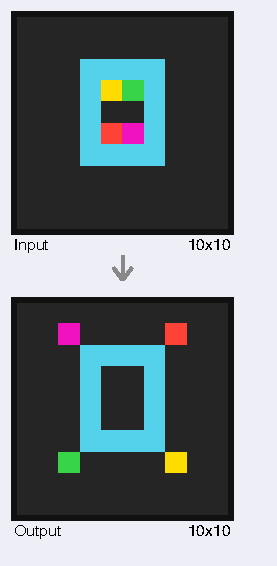
\includegraphics[width=\linewidth]{Figures/viz_task_pair.pdf}
        \small (a) Pair view
    \end{minipage}
    \hfill
    \begin{minipage}[c]{0.74\linewidth}
        \centering
        \begin{minipage}[b]{0.32\linewidth}
            \centering
            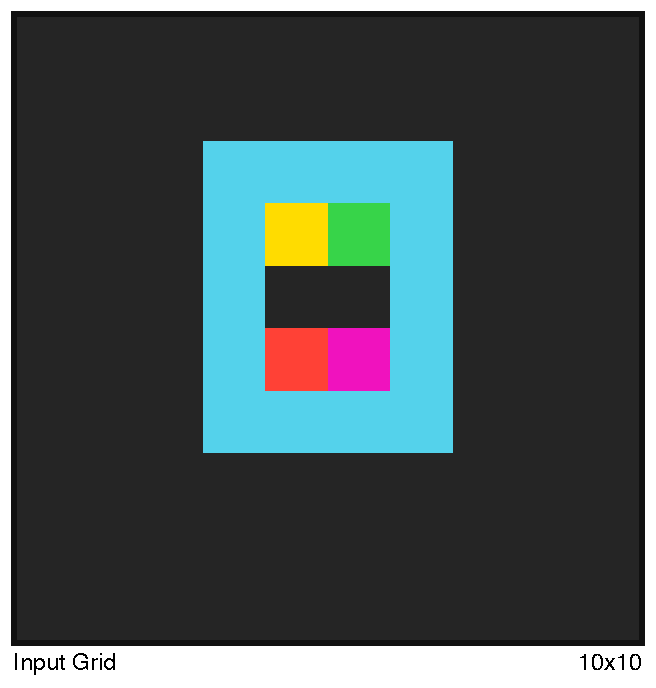
\includegraphics[width=\linewidth]{Figures/viz_single_grid.pdf}
            \small (b) Grid view
        \end{minipage}
        \hfill
        \begin{minipage}[b]{0.64\linewidth}
            \centering
            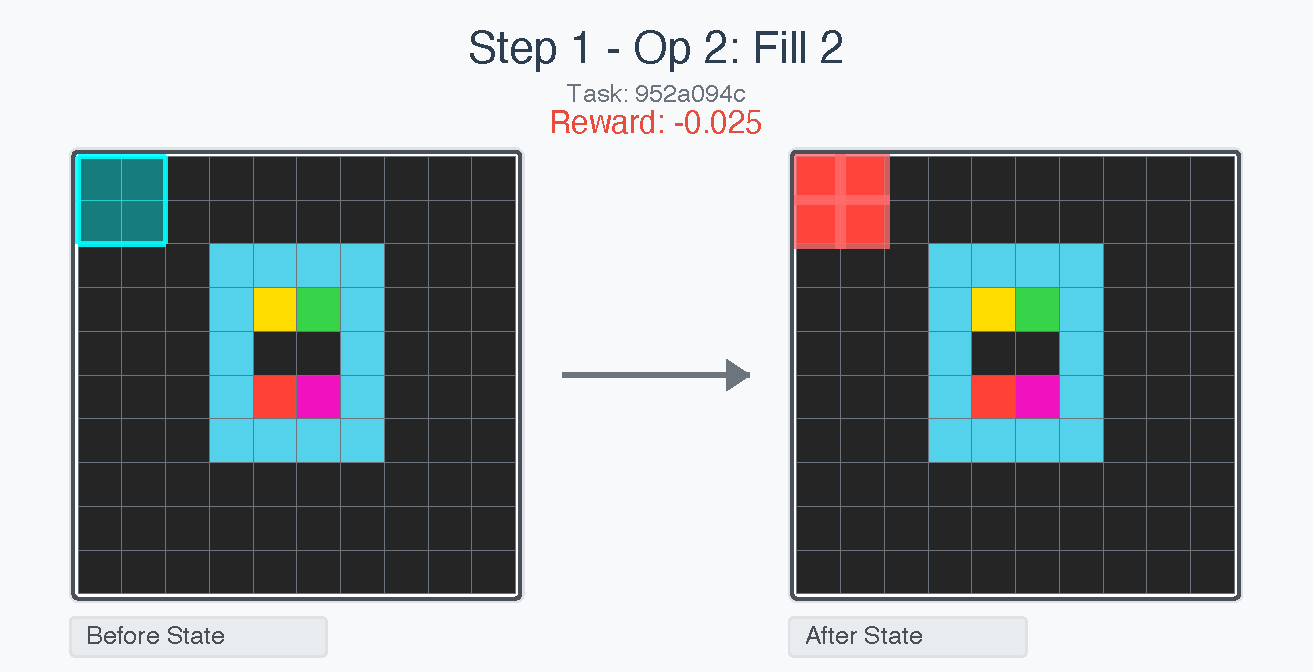
\includegraphics[width=\linewidth]{Figures/viz_rl_step.pdf}
            \small (c) Transition
        \end{minipage}

        \vspace{0.5em}

        \begin{minipage}[b]{0.98\linewidth}
            \centering
            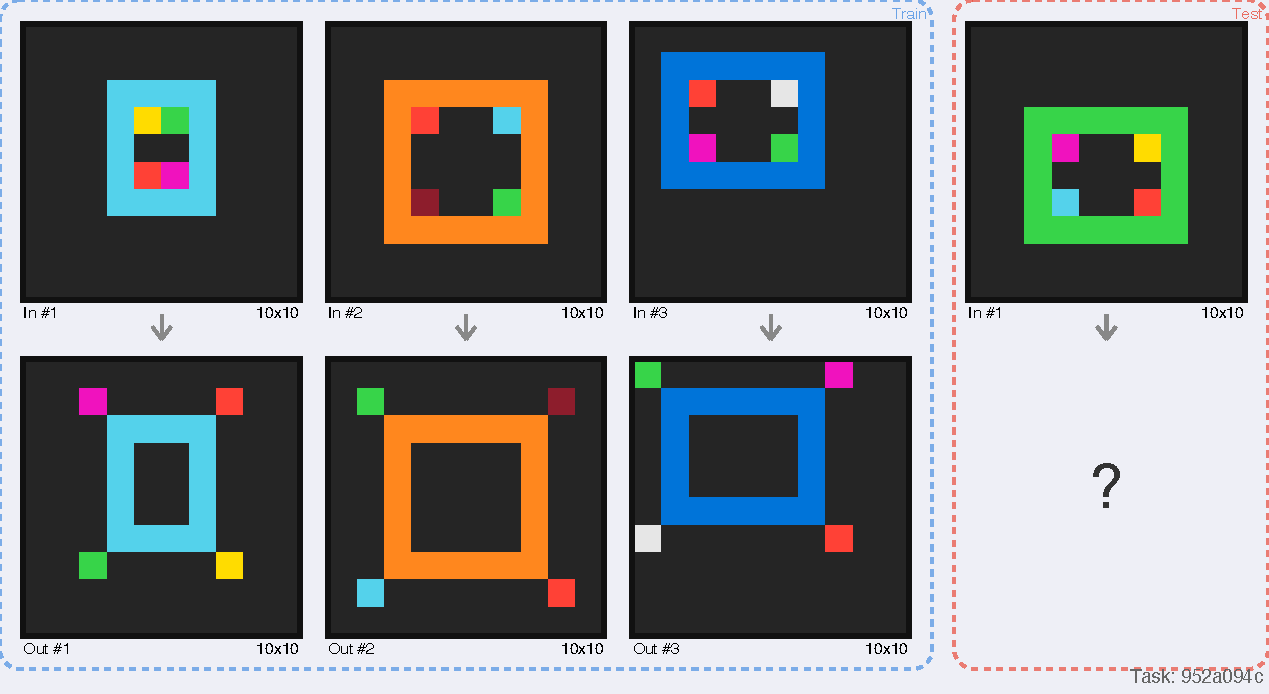
\includegraphics[width=\linewidth]{Figures/viz_complete_task.pdf}
            \small (d) Full task context
        \end{minipage}
    \end{minipage}
    \caption{Visualization modes in JaxARC. (a) A single input--output example. (b) A standalone grid. (c) A single RL step with action and reward annotations. (d) The complete task anatomy, showing support pairs and a held-out query.}
    \label{fig:viz_modes_appendix}
\end{figure}

\subsection{Internal data structures}
\label{app:data_structures}

JaxARC keeps a strict separation between immutable task data (\texttt{JaxArcTask}), static environment parameters (\texttt{EnvParams}), and the dynamic per-episode state (\texttt{State}). All three are Equinox PyTrees with statically-shaped leaves, so they can be freely passed through \texttt{jit}, \texttt{vmap}, and \texttt{pmap}. Table~\ref{tab:state_layout} lists the dynamic fields of \texttt{State}; the static parameters reside in \texttt{EnvParams} together with the stacked task buffer and the optional subset index view.

\begin{table}[htbp]
\centering
\caption{Dynamic per-episode state in JaxARC. All grids and masks are padded to the dataset's $H_{\max} \times W_{\max}$ canvas; counts apply to the active region defined by \texttt{working\_grid\_mask}.}
\label{tab:state_layout}
\scriptsize
\resizebox{\linewidth}{!}{%
\begin{tabular}{@{}lll@{}}
\toprule
\textbf{Field} & \textbf{Type / shape} & \textbf{Role} \\
\midrule
\texttt{working\_grid} & \texttt{int32[$H_{\max}, W_{\max}$]} & Current grid being edited (color values $0$--$9$) \\
\texttt{working\_grid\_mask} & \texttt{bool[$H_{\max}, W_{\max}$]} & Active cells of the working grid \\
\texttt{input\_grid}, \texttt{input\_grid\_mask} & same shapes & Original input grid for the active pair \\
\texttt{target\_grid}, \texttt{target\_grid\_mask} & same shapes & Target grid; masked to background in query mode \\
\texttt{selected} & \texttt{bool[$H_{\max}, W_{\max}$]} & Selection mask for the next operation \\
\texttt{clipboard} & \texttt{int32[$H_{\max}, W_{\max}$]} & Buffer for copy/paste operations \\
\texttt{step\_count} & \texttt{int32} & Current step within the episode \\
\texttt{task\_idx}, \texttt{pair\_idx} & \texttt{int32} & Indices into the task buffer \\
\texttt{allowed\_operations\_mask} & \texttt{bool[$35$]} & Currently enabled operations \\
\texttt{similarity\_score} & \texttt{float32} & Match between working and target grid \\
\texttt{key} & \texttt{uint32[$2$]} & Per-environment PRNG key \\
\bottomrule
\end{tabular}
}
\end{table}

The task buffer is a single stacked PyTree of \texttt{JaxArcTask} fields, prepared on the host and transferred to the device once. Each task entry stores up to \texttt{max\_train\_pairs} support pairs (default 10) and \texttt{max\_test\_pairs} query pairs (default 3), together with their boolean masks and an integer task identifier. Subset selection is implemented as an \texttt{int32} \texttt{subset\_indices} array that gathers from the full buffer, so subsets do not require recompilation.

\subsection{Reset and transition semantics}
\label{app:reset_and_step}

The compiled \texttt{reset} samples a task index from the active subset, samples a pair index uniformly from the available support or query pairs, and constructs the initial \texttt{State} via the working-grid initializer (Section~\ref{app:grid_init}). The \texttt{step} function performs four operations: (i) operation validation against the active operation profile, (ii) execution of the selected grid operation, (iii) computation of the new similarity score against the target grid, and (iv) emission of a Stoa \citep{toledoStoaJAXnativeInterface2025} \texttt{TimeStep} with one of three step types.

\begin{itemize}
    \item \texttt{TERMINATED} when the agent submits (operation $34$), regardless of whether the submission is correct.
    \item \texttt{TRUNCATED} when \texttt{step\_count} reaches \texttt{max\_episode\_steps} without a submission.
    \item \texttt{MID} otherwise.
\end{itemize}

The discount factor is set to $0$ on \texttt{TERMINATED} and \texttt{TRUNCATED} steps and to $1$ on \texttt{MID} steps. The episode mode (\texttt{train} vs \texttt{test}) is carried inside \texttt{EnvParams} rather than \texttt{State}, which allows the same compiled environment to be re-used for both visible-target rollouts and hidden-target evaluation by swapping \texttt{EnvParams}.

\paragraph{Reward components.} The submit-aware reward used by every profile is the sum
\begin{equation*}
    r_t = \alpha \,\Delta s_t \cdot \mathbb{1}[\text{train}]\;+\; c_{\text{step}}\;+\; b_{\text{succ}}\,\mathbb{1}[\text{submit} \wedge s_t = 1]\;+\; p_{\text{unsolved}}\,\mathbb{1}[\text{submit} \wedge s_t < 1],
\end{equation*}
where $s_t$ is the similarity score after the step, $\Delta s_t = s_t - s_{t-1}$ is its improvement, and the constants $\alpha, c_{\text{step}}, b_{\text{succ}}, p_{\text{unsolved}}$ are taken from the active reward profile (Section~\ref{app:reward_config}). Similarity shaping is automatically disabled in evaluation mode, where $\Delta s_t$ is multiplied by $\mathbb{1}[\text{train}]=0$, leaving only the step penalty, success bonus, and unsolved penalty.

\subsection{Grid similarity score}
\label{app:similarity}

Similarity is computed against the target grid's active region. Let $\mathcal{T}$ be the set of cells with \texttt{target\_grid\_mask}$=$true; the similarity is
\begin{equation*}
    s = \frac{1}{|\mathcal{T}|}\sum_{(i,j) \in \mathcal{T}} \mathbb{1}\!\left[\text{working}_{ij} = \text{target}_{ij}\;\wedge\;\text{working\_grid\_mask}_{ij}\right],
\end{equation*}
with $s = 1$ when both grids are empty and $s = 0$ when the target is empty but the working grid contains content. This definition penalizes both content mismatches and size mismatches: cells outside the target's active region or outside the working grid's active region count as incorrect, so an oversized or undersized submission cannot reach $s=1$. A solved episode requires $s=1$ at the moment the agent emits the \texttt{SUBMIT} operation; truncation alone never grants the success bonus.

\subsection{Working-grid initialization strategies}
\label{app:grid_init}

The initial working grid is sampled from a configurable mixture of four strategies. Weights need not sum to one; they are renormalized at compile time. Table~\ref{tab:grid_init} lists the strategies and their behavior. The baseline experiments use \texttt{demo\_weight}$=1.0$ (the remaining weights set to zero), which reproduces the standard ARC formulation in which the agent edits the input grid into the target output. Permutation, empty, and random initializers are intended for curriculum, robustness, and pre-training studies that go beyond the scope of this paper.

\begin{table}[htbp]
\centering
\caption{Working-grid initialization strategies. The agent is assigned one strategy per episode using the configured weights.}
\label{tab:grid_init}
\scriptsize
\resizebox{\linewidth}{!}{%
\begin{tabular}{@{}lll@{}}
\toprule
\textbf{Mode} & \textbf{Source} & \textbf{Behavior} \\
\midrule
\texttt{demo} & A randomly sampled support pair input & Standard ARC editing setup \\
\texttt{permutation} & Demo input with a random rotation, reflection, or color remap & Synthetic augmentation \\
\texttt{empty} & Padded zero grid with the dataset's grid mask & Pure ``construct from scratch'' setting \\
\texttt{random} & Sparse or dense Bernoulli pattern over the active mask & Robustness / noise probing \\
\bottomrule
\end{tabular}
}
\end{table}

\subsection{API usage examples}
\label{app:usage}

JaxARC follows the stateless API used by JAX environment libraries: random state is carried through explicit PRNG keys, and the environment state is a PyTree passed into and returned from each transition. Listing~\ref{lst:minimal_api} shows a single-task loop. Listing~\ref{lst:batched_api} shows the same reset and step functions under \texttt{vmap}.

\begin{lstlisting}[style=jaxarcpython, caption={Minimal transition loop for a single task.}, label={lst:minimal_api}]
import jax
from jaxarc import make

# Initialize environment and static parameters
env, env_params = make("Mini-Most_Common_color_l6ab0lf3xztbyxsu3p")

# Stateless reset
key = jax.random.PRNGKey(0)
state, timestep = env.reset(key, env_params=env_params)

action = env.action_space(env_params).sample(key)
state, timestep = env.step(state, action, env_params=env_params)
\end{lstlisting}

\begin{lstlisting}[style=jaxarcpython, caption={High-throughput vectorization using \texttt{vmap}.}, label={lst:batched_api}]
num_envs = 1024
keys = jax.random.split(jax.random.PRNGKey(0), num_envs)

# Batch the reset logic
reset_one = lambda k: env.reset(k, env_params=env_params)
states, timesteps = jax.jit(jax.vmap(reset_one))(keys)

# Batch the step logic
step_one = lambda s, a: env.step(s, a, env_params=env_params)
actions = jax.vmap(env.action_space(env_params).sample)(keys)
states, timesteps = jax.jit(jax.vmap(step_one))(states, actions)
\end{lstlisting}

\section{Datasets and task subsets}
\label{app:datasets}

JaxARC partitions the ARC problem space into datasets, each managed by a parser and registry entry. The parsers preserve ARC's native grid-size range ($1 \times 1$ to $30 \times 30$) while padding task tensors into fixed-shape accelerator buffers. A scenario selects the active task subset before compilation, for example \texttt{AGI1-entry} or \texttt{Concept-Count}. This keeps the compiled transition shape static while allowing the benchmark to report by task family.

\subsection{ARC-AGI-1 groups}
\label{app:arcagi_subsets}

For the ARC-AGI-1 sweep, we adopted the task tiers defined by the ARC-Game project at \url{https://github.com/volotat/ARC-Game/blob/main/tasks/levels.json}. While these labels provide a useful heterogeneous reporting structure, we emphasize that they are subjective and have not been formally calibrated for difficulty. Table~\ref{tab:agi1_subset_counts} lists the counts for each label used in this work; counts match the YAML subset files shipped with the JaxARC baseline configurations.

\begin{table}[htbp]
\centering
\caption{ARC-AGI-1 groupings used for benchmarking. Task counts are based on subjective ARC-Game labels.}
\label{tab:agi1_subset_counts}
\small
\begin{tabular}{@{}lr@{}}
\toprule
\textbf{Grouping} & \textbf{Tasks} \\
\midrule
\texttt{entry} & 33 \\
\texttt{easy} & 304 \\
\texttt{medium} & 263 \\
\texttt{hard} & 66 \\
\texttt{multiple\_solutions} & 33 \\
\texttt{tedious} & 73 \\
\bottomrule
\end{tabular}
\end{table}

\subsection{ConceptARC concept groups}
\label{app:concept_mini}

The ConceptARC benchmark is organized into concept groups that isolate specific spatial or logical rules. Our main baseline figure focuses on six representative groups: AboveBelow, Center, CleanUp, CompleteShape, Copy, and Count. The full 16-group breakdown is reported in Appendix~\ref{app:extended_baselines}.

\subsection{Extensibility and custom subsets}
\label{app:extensibility}

JaxARC is designed for easy extension to new task families and curated subsets. The \texttt{make} function provides a unified interface for instantiating environments from predefined groups, custom YAML files, or individual tasks.

\paragraph{Predefined subsets.}
To facilitate standard benchmarking, common task groupings are predefined and available immediately:
\begin{itemize}
    \item \textbf{ConceptARC:} All 16 concept groups are registered as subsets (e.g., \texttt{make("Concept-AboveBelow")}).
    \item \textbf{ARC-AGI:} The standard splits are available as \texttt{make("AGI1-train")} and \texttt{make("AGI1-eval")}.
    \item \textbf{Single tasks:} Any individual task can be isolated by appending its ID to the dataset key (e.g., \texttt{make("Mini-l6ab0lf3...")}). This is particularly useful for debugging specific reasoning failures.
\end{itemize}

\paragraph{YAML-based subsets.}
A common pattern for creating reproducible benchmarks is to define a subset in a YAML file. These files should be placed in the project configuration directory under \texttt{configs/env/jaxarc/subsets/\{Dataset\}/\{name\}.yaml}. Once the file is saved, the subset can be instantiated using the hyphenated identifier (e.g., \texttt{make("AGI1-my\_benchmark")}). Library users should first call \texttt{load\_all\_subsets\_for\_dataset("AGI1")} to discover these files at process start-up.

\paragraph{Programmatic registration.}
Subsets can also be registered at runtime without modifying the file system. This is useful for implementing curriculum learning or dynamically generating task groups during an experiment.

\begin{lstlisting}[style=jaxarcpython, caption={Programmatic subset registration and single-task instantiation.}]
from jaxarc.registration import register_subset, make

# 1. Register a custom task group
my_tasks = ["task_id_1", "task_id_2"]
register_subset("Mini", "custom_group", my_tasks)
env, params = make("Mini-custom_group")

# 2. Instantiate a single specific task
env, params = make("Mini-Most_Common_color_l6ab0lf3xztbyxsu3p")
\end{lstlisting}

\paragraph{Zero-config initialization and auto-download.}
To minimize setup friction, JaxARC includes an \texttt{auto\_download} parameter in the \texttt{make} function. When set to \texttt{True}, the environment registry detects if the required dataset files are missing from the local cache, fetches them from the official upstream repository, and organizes the files in the appropriate local directory before proceeding with environment creation.

\begin{lstlisting}[style=jaxarcpython, caption={Zero-config instantiation with automatic dataset acquisition.}]
from jaxarc.registration import make

# Automatically downloads AGI1 tasks if not present locally
env, params = make("AGI1-entry", auto_download=True)
\end{lstlisting}

For ARC-AGI datasets the registry performs cross-split lookups automatically: if a task ID is requested but not found in the current split (e.g., \texttt{train}), the system attempts to locate it in the opposite split (\texttt{evaluation}) before reporting an error. This makes it possible to define a custom subset that mixes IDs from both standard splits without writing a custom parser.

\section{Configuration surface}
\label{app:configuration_surface}

JaxARC exposes the main experimental degrees of freedom as explicit configuration axes. Table~\ref{tab:hydra_config_surface} summarizes these axes and the specific values used in our multi-algorithm baselines.

\begin{table}[htbp]
\centering
\caption{Experimental configuration surface in JaxARC.}
\label{tab:hydra_config_surface}
\scriptsize
\resizebox{\linewidth}{!}{%
\begin{tabular}{@{}lll@{}}
\toprule
\textbf{Axis} & \textbf{Value(s) used in this paper} & \textbf{Description} \\
\midrule
Dataset & ARC-AGI-1, ConceptARC, MiniARC & Source of raw JSON tasks \\
Scenario & e.g., \texttt{AGI1-entry}, \texttt{Concept-Count} & Active task subset selector \\
Action mode & \texttt{point} & Parameterization of the selection mask \\
Operation profile & \texttt{raw} (unless specified otherwise) & Allowed set of editing operations \\
Observation stack & answer, input, contextual & Configured grid channels for the policy \\
Reward profile & balanced & Shaping and submission rewards \\
Episode limit & 100 steps & Maximum edits before truncation \\
Grid initializer & \texttt{demo} (weight $1.0$) & Working grid copies the support input \\
Evaluation schedule & 20 intervals, 32 episodes each & Periodic monitoring during training \\
\bottomrule
\end{tabular}
}
\end{table}

\section{Interface and reward design}
\label{app:action_reward_config}

\subsection{Action wrappers}
\label{app:action_config}

The environment core receives an operation ID and a selection mask. To keep the action space tractable for discrete RL, we provide wrappers that simplify this interface. The \texttt{point} wrapper, used in our baselines, represents an action as $(\texttt{op}, \texttt{row}, \texttt{col})$, while the \texttt{bbox} wrapper accepts $(\texttt{op}, r_1, c_1, r_2, c_2)$ tuples that the wrapper materializes into a rectangular mask. A separate \texttt{FlattenActionWrapper} composes any nested \texttt{Dict}/\texttt{MultiDiscrete} action space into a single \texttt{Discrete} action so that off-the-shelf algorithm implementations can consume the interface without modification. Table~\ref{tab:action_profiles} lists the operation profiles available in the environment and Table~\ref{tab:operation_ids} the canonical operation IDs.

\begin{table}[htbp]
\centering
\caption{Operation profiles in JaxARC.}
\label{tab:action_profiles}
\scriptsize
\resizebox{\linewidth}{!}{%
\begin{tabular}{@{}lll@{}}
\toprule
\textbf{Profile} & \textbf{Op IDs} & \textbf{Functional categories} \\
\midrule
\texttt{raw} & 0--9, 33, 34 & Color fill, resize, submit \\
\texttt{standard} & 0--19, 28--34 & + Flood fill, clipboard, clear, copy input \\
\texttt{full} & 0--34 & + Movement, rotation, and geometric flips \\
\bottomrule
\end{tabular}
}
\end{table}

\begin{table}[htbp]
\centering
\caption{Canonical operation identifiers in JaxARC.}
\label{tab:operation_ids}
\scriptsize
\resizebox{\linewidth}{!}{%
\begin{tabular}{@{}lll@{}}
\toprule
\textbf{Range} & \textbf{Operations} & \textbf{Effect} \\
\midrule
0--9 & \texttt{FILL\_[0-9]} & Apply color to selection \\
10--19 & \texttt{FLOOD\_FILL\_[0-9]} & Flood fill from a single selected cell \\
20--23 & \texttt{MOVE\_[UP|DOWN|LEFT|RIGHT]} & Shift the selection's bounding box with wrap \\
24--25 & \texttt{ROTATE\_[C|CC]} & $90^\circ$ rotation of a square selection \\
26--27 & \texttt{FLIP\_[H|V]} & Reflect inside the selection's bounding box \\
28--30 & \texttt{COPY}, \texttt{PASTE}, \texttt{CUT} & Clipboard interaction \\
31--33 & \texttt{CLEAR}, \texttt{COPY\_INPUT}, \texttt{RESIZE} & Grid management \\
34 & \texttt{SUBMIT} & Terminate and evaluate \\
\bottomrule
\end{tabular}
}
\end{table}

\subsection{Operation semantics}
\label{app:op_semantics}

Several operations have implicit preconditions that affect how the policy can use them. Knowing them is important when comparing learning curves across operation profiles.

\begin{itemize}
    \item \textbf{Empty selection.} For object operations (movement, rotation, flip), an empty selection mask is replaced by the working-grid mask, so the action acts on the entire active grid. For clipboard, fill, and flood-fill operations, an empty selection is a no-op.
    \item \textbf{Bounding-box semantics.} \texttt{MOVE}, \texttt{ROTATE}, and \texttt{FLIP} act on the axis-aligned bounding box of the selection rather than on the individual selected cells. Movement wraps inside that bounding box.
    \item \textbf{Single-cell flood fill.} \texttt{FLOOD\_FILL\_[0-9]} requires exactly one selected cell. It is silently skipped if the selection contains zero or multiple cells; this avoids ambiguity over which seed pixel to use.
    \item \textbf{Square rotation.} \texttt{ROTATE\_C} and \texttt{ROTATE\_CC} only execute when the selection's bounding box is square. Non-square requests are no-ops.
    \item \textbf{Resize.} The bottom-right cell of the selection defines the new active grid size relative to the top-left corner $(0,0)$. Existing content within the new region is preserved; newly active cells are filled with color $0$.
    \item \textbf{Submit.} \texttt{SUBMIT} terminates the episode unconditionally. The success bonus is granted only if $s=1$ at submission time.
\end{itemize}

\subsection{Observation channels}
\label{app:observation_wrappers}

The base observation is the current working grid. Observation wrappers concatenate additional grid channels for task context. This design lets the same environment expose diagnostic interfaces, such as answer-visible positive controls, without changing the transition function. Table~\ref{tab:observation_wrappers} lists the wrappers used to build the observation stack. Stacks are composable: the baseline policy uses the working grid plus the input, the (target-mode-aware) answer, and five contextual support pairs, for a total of $13$ channels at $30 \times 30$. Wrappers can be combined in any order; channel counts are additive.

\begin{table}[htbp]
\centering
\caption{Observation wrappers. Channel counts are additive to the base working grid.}
\label{tab:observation_wrappers}
\scriptsize
\resizebox{\linewidth}{!}{%
\begin{tabular}{@{}lcl@{}}
\toprule
\textbf{Wrapper} & \textbf{Channels} & \textbf{Content} \\
\midrule
\texttt{InputGridObservationWrapper} & 1 & The original input grid for the active pair \\
\texttt{AnswerObservationWrapper} & 1 & Target grid (masked to background in query mode) \\
\texttt{ContextualObservationWrapper} & $2N$ & $N$ support input/output pairs (default $N{=}5$) \\
\texttt{ClipboardObservationWrapper} & 1 & Current clipboard contents \\
\bottomrule
\end{tabular}
}
\end{table}

The contextual wrapper draws from the task buffer rather than the policy state, so the additional channels never depend on transient information that could leak the target. In training (support) mode, the wrapper excludes the active pair from the context to prevent the policy from trivially copying the answer it is currently asked to produce.

\subsection{Reward profiles}
\label{app:reward_config}

Rewards are the sum of scalar penalties and bonuses, as defined in Section~\ref{app:reset_and_step}. The \texttt{balanced} profile used for the reported baselines includes a dense similarity term, which gives shallow model-free agents a learning signal while they explore the editing interface. When evaluating hidden-target submissions, the evaluator can disable this similarity term so that reward does not reveal target-grid information.

\begin{table}[htbp]
\centering
\caption{Scalar reward components in JaxARC profiles. Similarity reward is multiplied by an indicator that is zero in evaluation mode.}
\label{tab:reward_profiles}
\scriptsize
\resizebox{\linewidth}{!}{%
\begin{tabular}{@{}lrrrrl@{}}
\toprule
\textbf{Profile} & \textbf{Step} & \textbf{Success} & \textbf{Unsolved} & \textbf{Similarity} & \textbf{Typical use} \\
\midrule
Balanced & $-0.02$ & $10.0$ & $-1.0$ & $1.0$ & Baseline benchmark sweep \\
Training & $-0.005$ & $10.0$ & $-1.0$ & $1.0$ & Dense-reward training \\
Evaluation & $-0.02$ & $10.0$ & $-1.0$ & $0.0$ & Hidden-target evaluation \\
\bottomrule
\end{tabular}
}
\end{table}

\section{Baseline experimental protocol}
\label{app:stoix}

JaxARC integrates with the Stoix framework \citep{toledoStoixDistributedSingleagent2024} through the \texttt{jaxarc.stoix\_adapter.make\_jaxarc\_env} factory, which composes the JaxARC action and observation wrappers with the standard Stoix wrapper chain. Listing~\ref{lst:wrapper_chain} describes the order of wrappers applied to every environment used in this paper; the order is significant because \texttt{AutoResetWrapper} relies on the metric wrappers having already finalized episode statistics for the just-completed episode.

\begin{lstlisting}[style=jaxarcpython, caption={Wrapper chain composed around the JaxARC core for the baseline sweep.}, label={lst:wrapper_chain}]
# 1. JaxARC core: action and observation wrappers
env = PointActionWrapper(env)            # (op, row, col) -> mask Action
env = FlattenActionWrapper(env)          # Dict/MultiDiscrete -> Discrete
env = AnswerObservationWrapper(env)      # +1 channel (target, mode-aware)
env = InputGridObservationWrapper(env)   # +1 channel (input grid)
env = ContextualObservationWrapper(env)  # +2N channels (support pairs)

# 2. Stoix core wrapper chain
env = AddRNGKey(env)
env = RecordEpisodeMetrics(env)
env = ExtendedMetrics(env)               # adds success/similarity tracking
env = AutoResetWrapper(env)
env = VmapWrapper(env)
\end{lstlisting}

The sweep consists of $4$ algorithms $\times$ $35$ subsets $\times$ $5$ seeds $= 700$ training runs. It covers $16$ ConceptARC concept groups and $19$ ARC-AGI-1 train, eval, or label-based subsets. With a budget of $10^7$ environment steps per run, the full sweep amounts to $7\times 10^9$ environment steps. We report learning curves for the full set of runs in Appendix~\ref{app:extended_baselines}. Table~\ref{tab:baseline_common_settings} summarizes the common settings across these runs.

\begin{table}[htbp]
\centering
\caption{Common benchmark settings for the multi-algorithm sweep.}
\label{tab:baseline_common_settings}
\small
\begin{tabular}{@{}ll@{}}
\toprule
\textbf{Parameter} & \textbf{Value} \\
\midrule
Training budget & $10^7$ environment steps per run \\
Runs per condition & 5 random seeds \\
Parallelization & 512 environments per run \\
Episode limit & 100 steps \\
Network architecture & Shallow CNN (2-layer torso) \\
Action interface & \texttt{point} actions (\texttt{raw} profile) \\
Observation interface & Working grid + input + context + visible answer \\
Reward profile & balanced \\
Grid initializer & \texttt{demo} mode only \\
Evaluation & 20 evaluations, 32 episodes per evaluation \\
\bottomrule
\end{tabular}
\end{table}

\subsection{Algorithm hyperparameters}
\label{app:baseline_hyperparameters}

Hyperparameters for the baseline multi-algorithm sweep are detailed in Table~\ref{tab:algorithm_hyperparams}. Values were selected for stable execution across many task families rather than tuned as per-task upper bounds. PPO follows the Stoix \texttt{ppo/ff\_ppo} default with our subset-benchmark overrides (rollout length, epoch count, minibatches, learning-rate decay disabled). DDQN uses the online network for action selection and the target network for value evaluation in the Q-learning target. PQN uses Q$(\lambda)$ targets with no replay buffer and a linearly decayed exploration schedule that anneals $\epsilon$ from $1.0$ to $0.1$ over the first half of training. REINFORCE uses an actor--critic variant with on-policy advantages and an entropy bonus.

\begin{table}[htbp]
\centering
\caption{Hyperparameters for baseline RL algorithms.}
\label{tab:algorithm_hyperparams}
\scriptsize
\begin{tabular}{@{}lllll@{}}
\toprule
\textbf{Hyperparameter} & \textbf{PPO} & \textbf{DDQN} & \textbf{PQN} & \textbf{REINFORCE} \\
\midrule
Learning rate & $3\!\cdot\!10^{-4}$ & $5\!\cdot\!10^{-4}$ & $5\!\cdot\!10^{-4}$ & $3\!\cdot\!10^{-4}$ \\
Rollout length & 25 & 2 & 8 & 32 \\
Epochs per update & 4 & 16 & 4 & n/a \\
Minibatches & 8 & n/a & 16 & n/a \\
Discount ($\gamma$) & 0.99 & 0.99 & 0.99 & 0.99 \\
Advantage estimation & GAE($\lambda{=}0.95$) & n/a & Q($\lambda{=}0.95$) & n/a \\
Replay buffer & n/a & $10^6$ transitions & none & n/a \\
Target update ($\tau$) & n/a & $0.005$ & n/a & n/a \\
Entropy regularization & 0.01 & n/a & n/a & 0.001 \\
Value weight & 0.5 & n/a & n/a & 1.0 \\
Exploration & Policy entropy & $\epsilon{=}0.1$ & $\epsilon$-decay $1.0\!\to\!0.1$ & Policy entropy \\
Gradient clip & 0.5 & 0.5 & 0.5 & 0.5 \\
Learning-rate decay & off & off & off & off \\
\bottomrule
\end{tabular}
\end{table}

\subsection{Network architecture}
\label{app:network_architecture}

The feedforward baselines use a shallow convolutional network. The actor and critic torsos each contain two $3\times3$ convolutional layers with $32$ channels, stride $1$, SiLU activations, no layer normalization, and two fully connected layers of width $128$ before the action or value head. Inputs are arranged as $H{\times}W{\times}C$ tensors (\texttt{channel\_first}$=$\texttt{False}) so that the JaxARC observation wrappers' channel concatenation is consumed without transposition. This architecture keeps the benchmark tractable across algorithms, subsets, and seeds. Stronger architectures may change both absolute performance and algorithm ordering.

\subsection{Episode metrics}
\label{app:episode_metrics}

The \texttt{ExtendedMetrics} wrapper inserted in the chain (Listing~\ref{lst:wrapper_chain}) tracks five additional per-episode statistics, accumulated across the rollout and committed to the metrics dictionary at the moment the episode terminates: \texttt{best\_similarity} (the maximum similarity reached at any step), \texttt{solved} (a boolean for $s=1$ at submission), \texttt{steps\_to\_solve} (the step index of the first $s=1$ event, $0$ otherwise), \texttt{final\_similarity} (the similarity score at the terminal step), and \texttt{was\_truncated} (whether the episode ended via the step limit). A small post-processing function turns these per-episode tensors into the aggregated quantities reported in the curves: \emph{success rate}, \emph{average steps to solve} over solved episodes, \emph{truncation rate}, and the mean of \texttt{best\_similarity} and \texttt{final\_similarity}.

\subsection{Compute and software environment}
\label{app:compute_env}

All baseline runs were executed with the JaxARC distribution at the project's pinned commit, the \texttt{stoix} fork shipped in the baselines repository, and JAX with the CUDA backend. Each run used a single NVIDIA H100 GPU with 80\,GB of memory and $512$ vectorized environments. With this configuration, a $10^7$-step run takes on the order of one to two hours of wall-clock time depending on the algorithm; the full $700$-run sweep was scheduled through the \texttt{jaxarc\_experiments.yaml} launcher with a maximum of four concurrent jobs per node. Throughput-benchmark measurements were taken on a separate set of devices (Apple M2 Pro, NVIDIA RTX 3090, NVIDIA H100) under the protocol of Section~\ref{app:throughput}. The pinned software environment used for the throughput benchmark is Python 3.13.5, JAX 0.6.2, NumPy 2.3.1, and Gymnasium 1.2.0; ARCLE was used at \texttt{ARCLE/RawARCEnv-v0} with \texttt{MiniARCLoader}.

\section{Throughput benchmark protocol}
\label{app:throughput}

The throughput benchmark uses MiniARC task \texttt{Most\_Common\_color\_l6ab0lf3xztbyxsu3p}. Each measurement executes $100$ steps per environment with automatic reset on episode termination. JaxARC timings exclude one-time JIT compilation and measure steady-state rollout time. ARCLE is measured without a compilation phase in synchronous and asynchronous Gymnasium vectorized modes. The hardware platforms are an Apple M2 Pro CPU, an NVIDIA RTX 3090 GPU, and an NVIDIA H100 GPU. ARCLE used \texttt{ARCLE/RawARCEnv-v0} with \texttt{MiniARCLoader} and a $5{\times}5$ maximum grid size in the matched benchmark, mirroring JaxARC's MiniARC configuration so that no framework is penalized by an oversized canvas.

\begin{figure}[htbp]
\centering
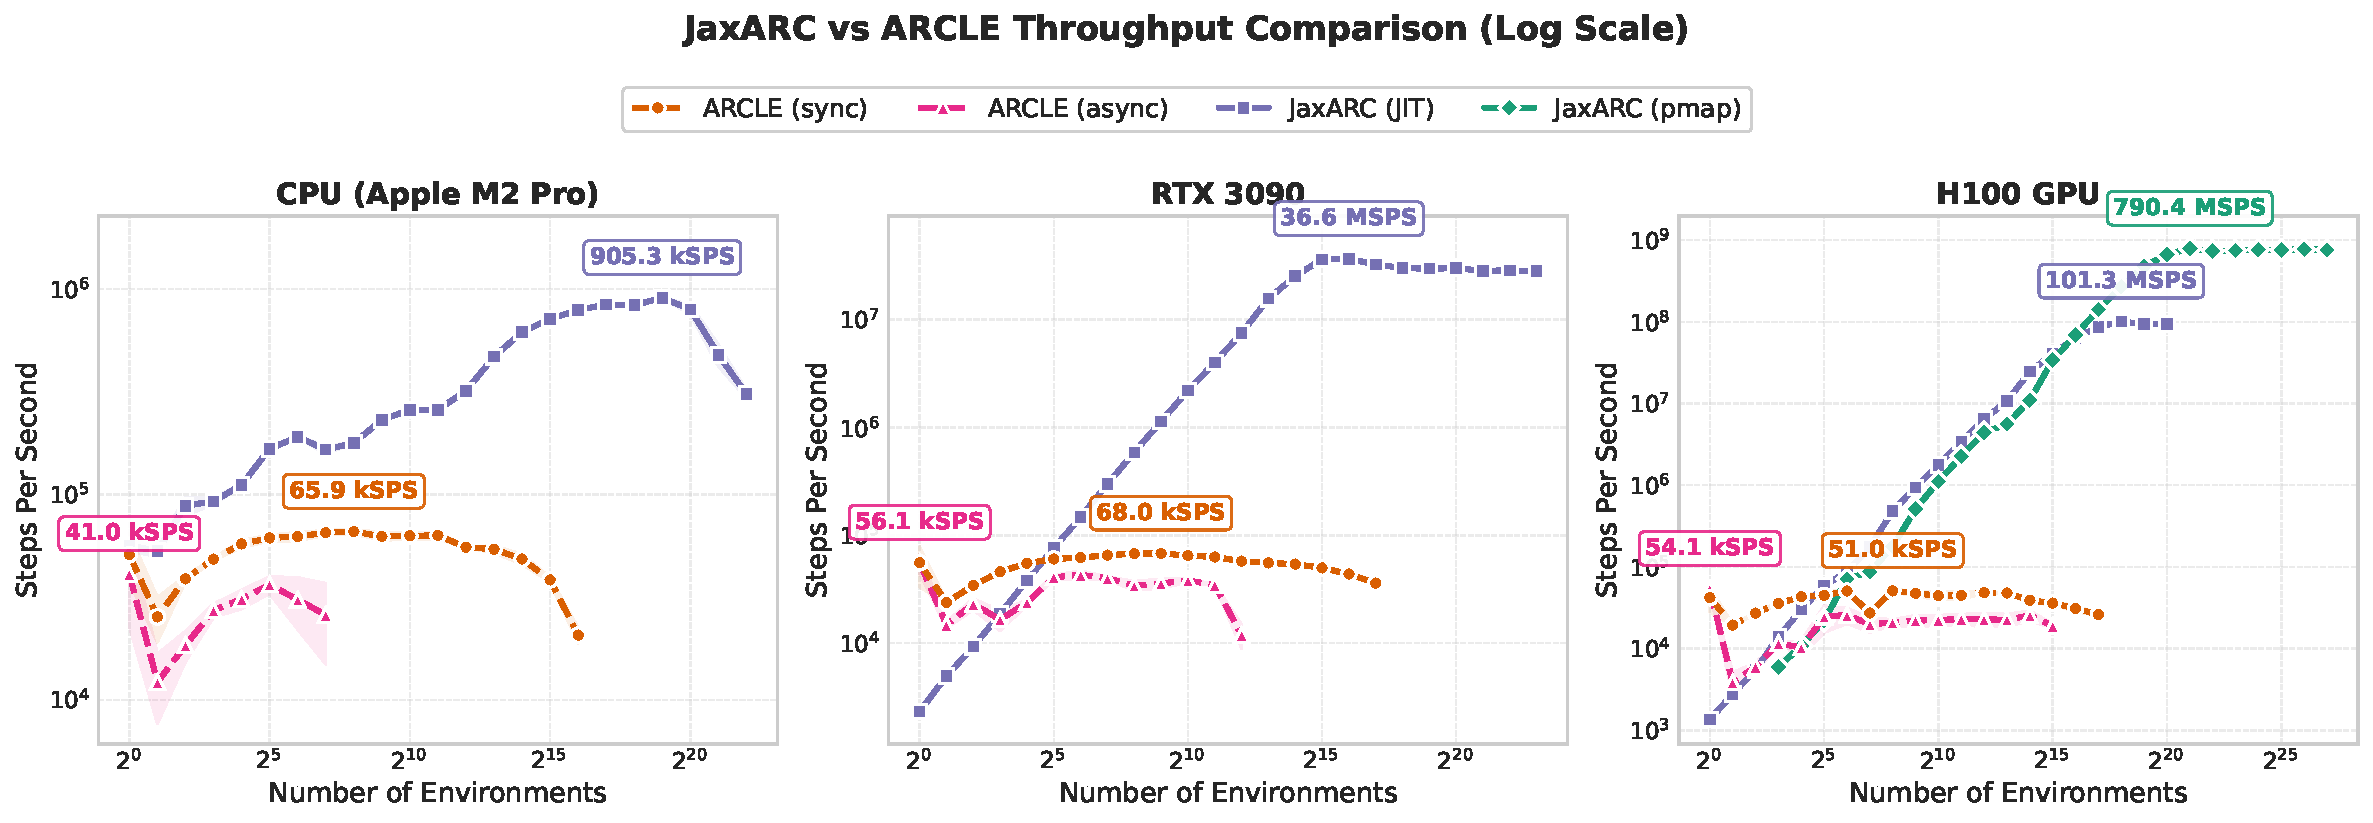
\includegraphics[width=0.95\linewidth]{Figures/throughput_combined_log.pdf}
\caption{Log-scale throughput across hardware platforms. The log scale reveals the crossover point where accelerator-native batching amortizes dispatch costs.}
\label{fig:throughput_log_appendix}
\end{figure}

Detailed speedup comparisons for each hardware tier are provided in Tables~\ref{tab:speedup_cpu_m2_pro}, \ref{tab:speedup_rtx_3090}, and \ref{tab:speedup_h100_gpu}. The H100 JIT run continues beyond the largest matched ARCLE batch and peaks at $101.3$M SPS at batch size $262{,}144$. A separate multi-device \texttt{pmap} benchmark reaches $790.4$M SPS at batch size $2{,}097{,}152$ and gives a $5{,}438.8\times$ speedup at the largest ARCLE-matched batch. We report the multi-device numbers separately because they require eight GPUs and are not directly comparable to ARCLE's CPU-only execution model; the matched-batch single-device numbers in the main results table provide the conservative comparison.

\begin{table}[htbp]
\centering
\caption{Detailed speedup comparison on CPU (M2 Pro)}
\label{tab:speedup_cpu_m2_pro}
\small
\begin{tabular}{lrrrrr}
\toprule
Batch Size & JaxARC SPS & Mode & ARCLE SPS & Mode & Speedup \\
\midrule
1 & 56,266 & jaxarc-jit & 50,823 & arcle-sync & 1.1$\times$ \\
2 & 53,035 & jaxarc-jit & 25,299 & arcle-sync & 2.1$\times$ \\
4 & 87,928 & jaxarc-jit & 38,816 & arcle-sync & 2.3$\times$ \\
8 & 92,525 & jaxarc-jit & 48,384 & arcle-sync & 1.9$\times$ \\
16 & 111,057 & jaxarc-jit & 57,336 & arcle-sync & 1.9$\times$ \\
32 & 166,687 & jaxarc-jit & 61,319 & arcle-sync & 2.7$\times$ \\
64 & 190,381 & jaxarc-jit & 62,324 & arcle-sync & 3.1$\times$ \\
128 & 165,107 & jaxarc-jit & 65,020 & arcle-sync & 2.5$\times$ \\
256 & 177,682 & jaxarc-jit & 65,871 & arcle-sync & 2.7$\times$ \\
512 & 230,453 & jaxarc-jit & 62,397 & arcle-sync & 3.7$\times$ \\
1,024 & 257,889 & jaxarc-jit & 62,820 & arcle-sync & 4.1$\times$ \\
2,048 & 257,877 & jaxarc-jit & 63,111 & arcle-sync & 4.1$\times$ \\
4,096 & 319,194 & jaxarc-jit & 55,270 & arcle-sync & 5.8$\times$ \\
8,192 & 467,960 & jaxarc-jit & 54,033 & arcle-sync & 8.7$\times$ \\
16,384 & 616,683 & jaxarc-jit & 48,383 & arcle-sync & 12.7$\times$ \\
32,768 & 714,731 & jaxarc-jit & 38,334 & arcle-sync & 18.6$\times$ \\
65,536 & 788,855 & jaxarc-jit & 20,634 & arcle-sync & 38.2$\times$ \\
\bottomrule
\end{tabular}
\end{table}

\begin{table}[htbp]
\centering
\caption{Detailed speedup comparison on RTX 3090}
\label{tab:speedup_rtx_3090}
\small
\begin{tabular}{lrrrrr}
\toprule
Batch Size & JaxARC SPS & Mode & ARCLE SPS & Mode & Speedup \\
\midrule
1 & 2,327 & jaxarc-jit & 56,066 & arcle-async & 0.0$\times$ \\
2 & 4,948 & jaxarc-jit & 23,845 & arcle-sync & 0.2$\times$ \\
4 & 9,282 & jaxarc-jit & 34,396 & arcle-sync & 0.3$\times$ \\
8 & 18,667 & jaxarc-jit & 45,991 & arcle-sync & 0.4$\times$ \\
16 & 38,305 & jaxarc-jit & 55,162 & arcle-sync & 0.7$\times$ \\
32 & 76,158 & jaxarc-jit & 60,394 & arcle-sync & 1.3$\times$ \\
64 & 147,835 & jaxarc-jit & 62,266 & arcle-sync & 2.4$\times$ \\
128 & 299,201 & jaxarc-jit & 65,513 & arcle-sync & 4.6$\times$ \\
256 & 589,248 & jaxarc-jit & 67,777 & arcle-sync & 8.7$\times$ \\
512 & 1,141,716 & jaxarc-jit & 68,011 & arcle-sync & 16.8$\times$ \\
1,024 & 2,205,416 & jaxarc-jit & 65,038 & arcle-sync & 33.9$\times$ \\
2,048 & 4,010,852 & jaxarc-jit & 63,005 & arcle-sync & 63.7$\times$ \\
4,096 & 7,519,602 & jaxarc-jit & 57,698 & arcle-sync & 130.3$\times$ \\
8,192 & 15,672,773 & jaxarc-jit & 55,584 & arcle-sync & 282.0$\times$ \\
16,384 & 25,365,090 & jaxarc-jit & 54,126 & arcle-sync & 468.6$\times$ \\
32,768 & 36,337,555 & jaxarc-jit & 50,002 & arcle-sync & 726.7$\times$ \\
65,536 & 36,570,507 & jaxarc-jit & 43,765 & arcle-sync & 835.6$\times$ \\
131,072 & 32,613,474 & jaxarc-jit & 36,131 & arcle-sync & 902.6$\times$ \\
\bottomrule
\end{tabular}
\end{table}

\begin{table}[htbp]
\centering
\caption{Detailed speedup comparison on H100 GPU}
\label{tab:speedup_h100_gpu}
\small
\begin{tabular}{lrrrrr}
\toprule
Batch Size & JaxARC SPS & Mode & ARCLE SPS & Mode & Speedup \\
\midrule
1 & 1,359 & jaxarc-jit & 54,082 & arcle-async & 0.0$\times$ \\
2 & 2,776 & jaxarc-jit & 19,375 & arcle-sync & 0.1$\times$ \\
4 & 5,482 & jaxarc-jit & 27,123 & arcle-sync & 0.2$\times$ \\
8 & 13,912 & jaxarc-jit & 35,775 & arcle-sync & 0.4$\times$ \\
16 & 30,045 & jaxarc-jit & 43,116 & arcle-sync & 0.7$\times$ \\
32 & 59,176 & jaxarc-jit & 44,860 & arcle-sync & 1.3$\times$ \\
64 & 86,458 & jaxarc-jit & 50,575 & arcle-sync & 1.7$\times$ \\
128 & 176,671 & jaxarc-jit & 27,236 & arcle-sync & 6.5$\times$ \\
256 & 482,233 & jaxarc-jit & 51,035 & arcle-sync & 9.4$\times$ \\
512 & 942,287 & jaxarc-jit & 47,571 & arcle-sync & 19.8$\times$ \\
1,024 & 1,766,400 & jaxarc-jit & 44,436 & arcle-sync & 39.8$\times$ \\
2,048 & 3,448,222 & jaxarc-jit & 44,965 & arcle-sync & 76.7$\times$ \\
4,096 & 6,440,953 & jaxarc-jit & 48,389 & arcle-sync & 133.1$\times$ \\
8,192 & 10,743,903 & jaxarc-jit & 47,972 & arcle-sync & 224.0$\times$ \\
16,384 & 24,598,104 & jaxarc-jit & 39,065 & arcle-sync & 629.7$\times$ \\
32,768 & 40,676,131 & jaxarc-jit & 36,002 & arcle-sync & 1129.8$\times$ \\
65,536 & 69,422,302 & jaxarc-pmap & 31,038 & arcle-sync & 2236.7$\times$ \\
131,072 & 141,892,015 & jaxarc-pmap & 26,089 & arcle-sync & 5438.8$\times$ \\
\bottomrule
\end{tabular}
\end{table}

\section{Extended baseline results}
\label{app:extended_baselines}

The extended baseline figures separate shaped editing progress from exact task solving. Episodic return increases on several ARC-AGI and ConceptARC subsets, especially for PPO, but exact success remains substantially lower. This gap indicates that the agents often learn partial edits, reward-shaping behavior, or frequent submissions without reliably producing the full target grid.

Across ARC-AGI groupings, PPO is strongest, REINFORCE is usually the closest competitor, and the value-based methods remain lower or less stable across most panels. ConceptARC shows larger variation across concept groups. Count is the clearest positive case for the shallow-CNN policy-gradient agents, while DDQN shows an early shaped-return gain on Count that does not persist through the full run. Several other groups show moderate shaped return with much weaker exact success. These per-family curves are therefore more informative than a single aggregate score, which would mix qualitatively different learning regimes.

The success-rate panel (Figure~\ref{fig:combined_success_rate}) is the strict measure consistent with the official ARC scoring rule. Reading it together with the episodic-return panels makes the gap between shaping progress and exact submission visible at the per-subset level, and clarifies which subsets remain open problems even for algorithms whose shaped return curves trend upward.

\begin{figure}[htbp]
\centering
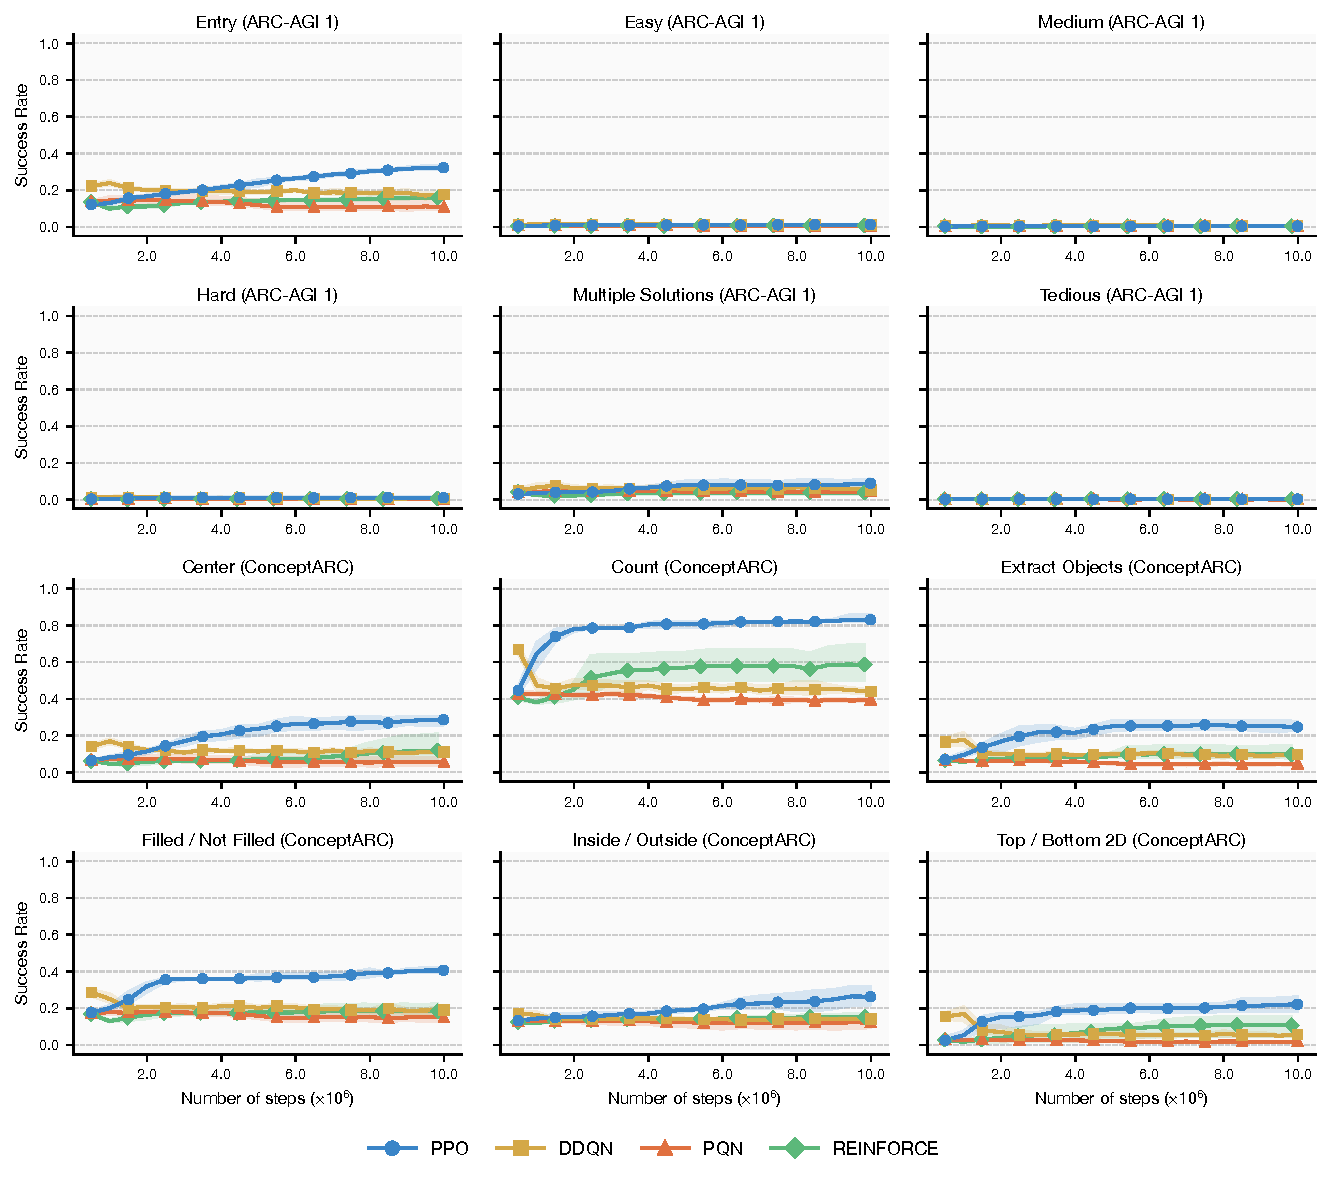
\includegraphics[width=0.95\linewidth]{Figures/combined_success_rate.pdf}
\caption{Success rates across the baseline sweep. Success is a binary, pixel-perfect metric and is significantly harder than optimizing shaped return.}
\label{fig:combined_success_rate}
\end{figure}

\begin{figure}[htbp]
\centering
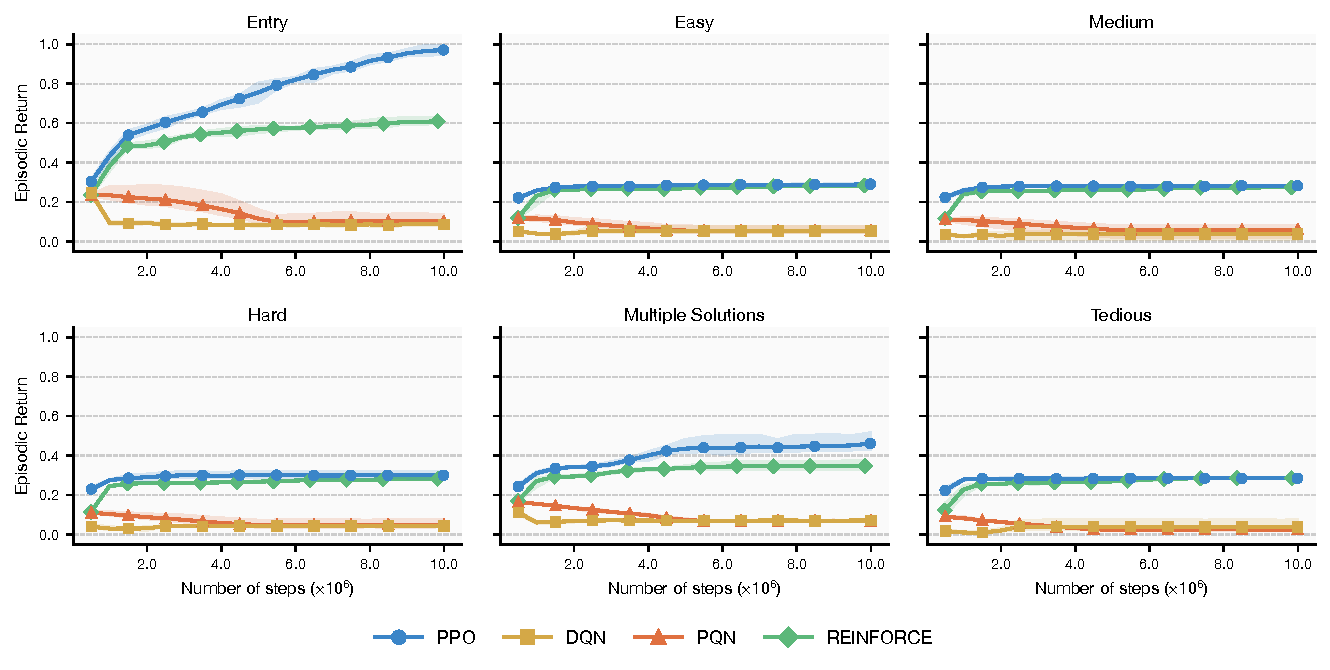
\includegraphics[width=0.95\linewidth]{Figures/arcagi1_episode_return.pdf}
\caption{Episodic return across ARC-AGI-1 groupings. The grouping names are subjective ARC-Game labels rather than official ARC-AGI difficulty levels.}
\label{fig:agi1_episode_return_full}
\end{figure}

\begin{figure}[htbp]
\centering
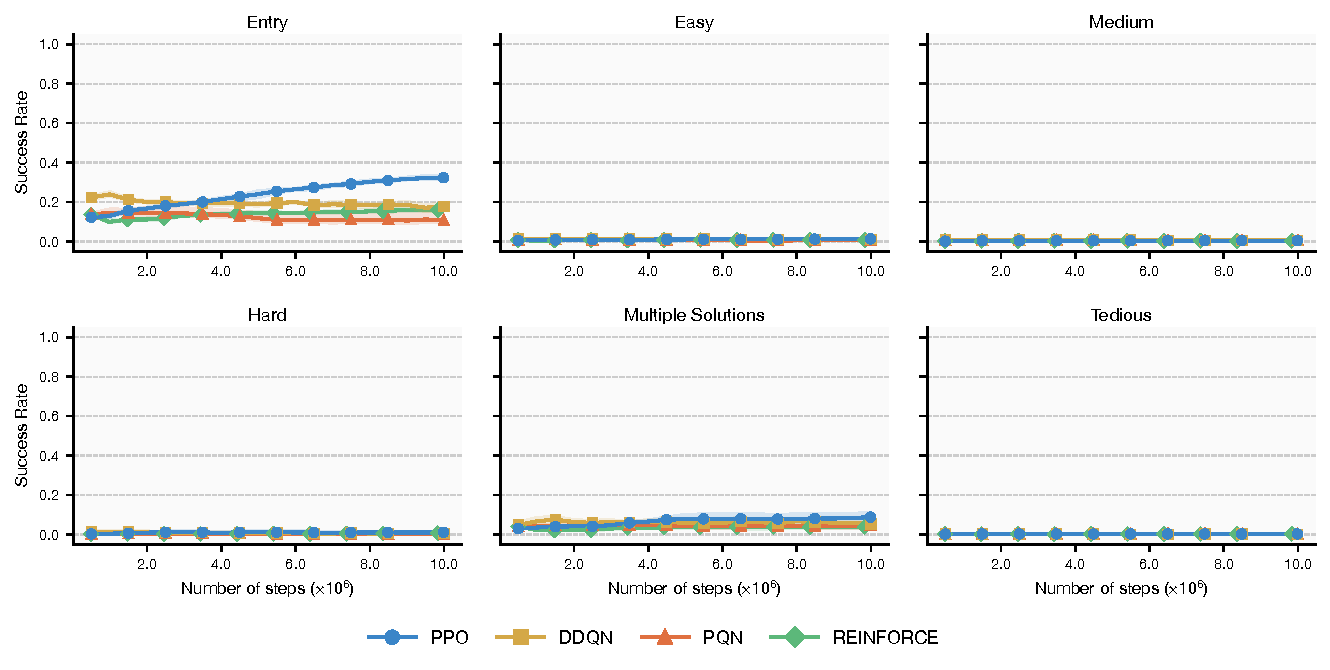
\includegraphics[width=0.95\linewidth]{Figures/arcagi1_success_rate.pdf}
\caption{Success rate across ARC-AGI-1 groupings.}
\label{fig:agi1_success_rate_full}
\end{figure}

\begin{figure}[htbp]
\centering
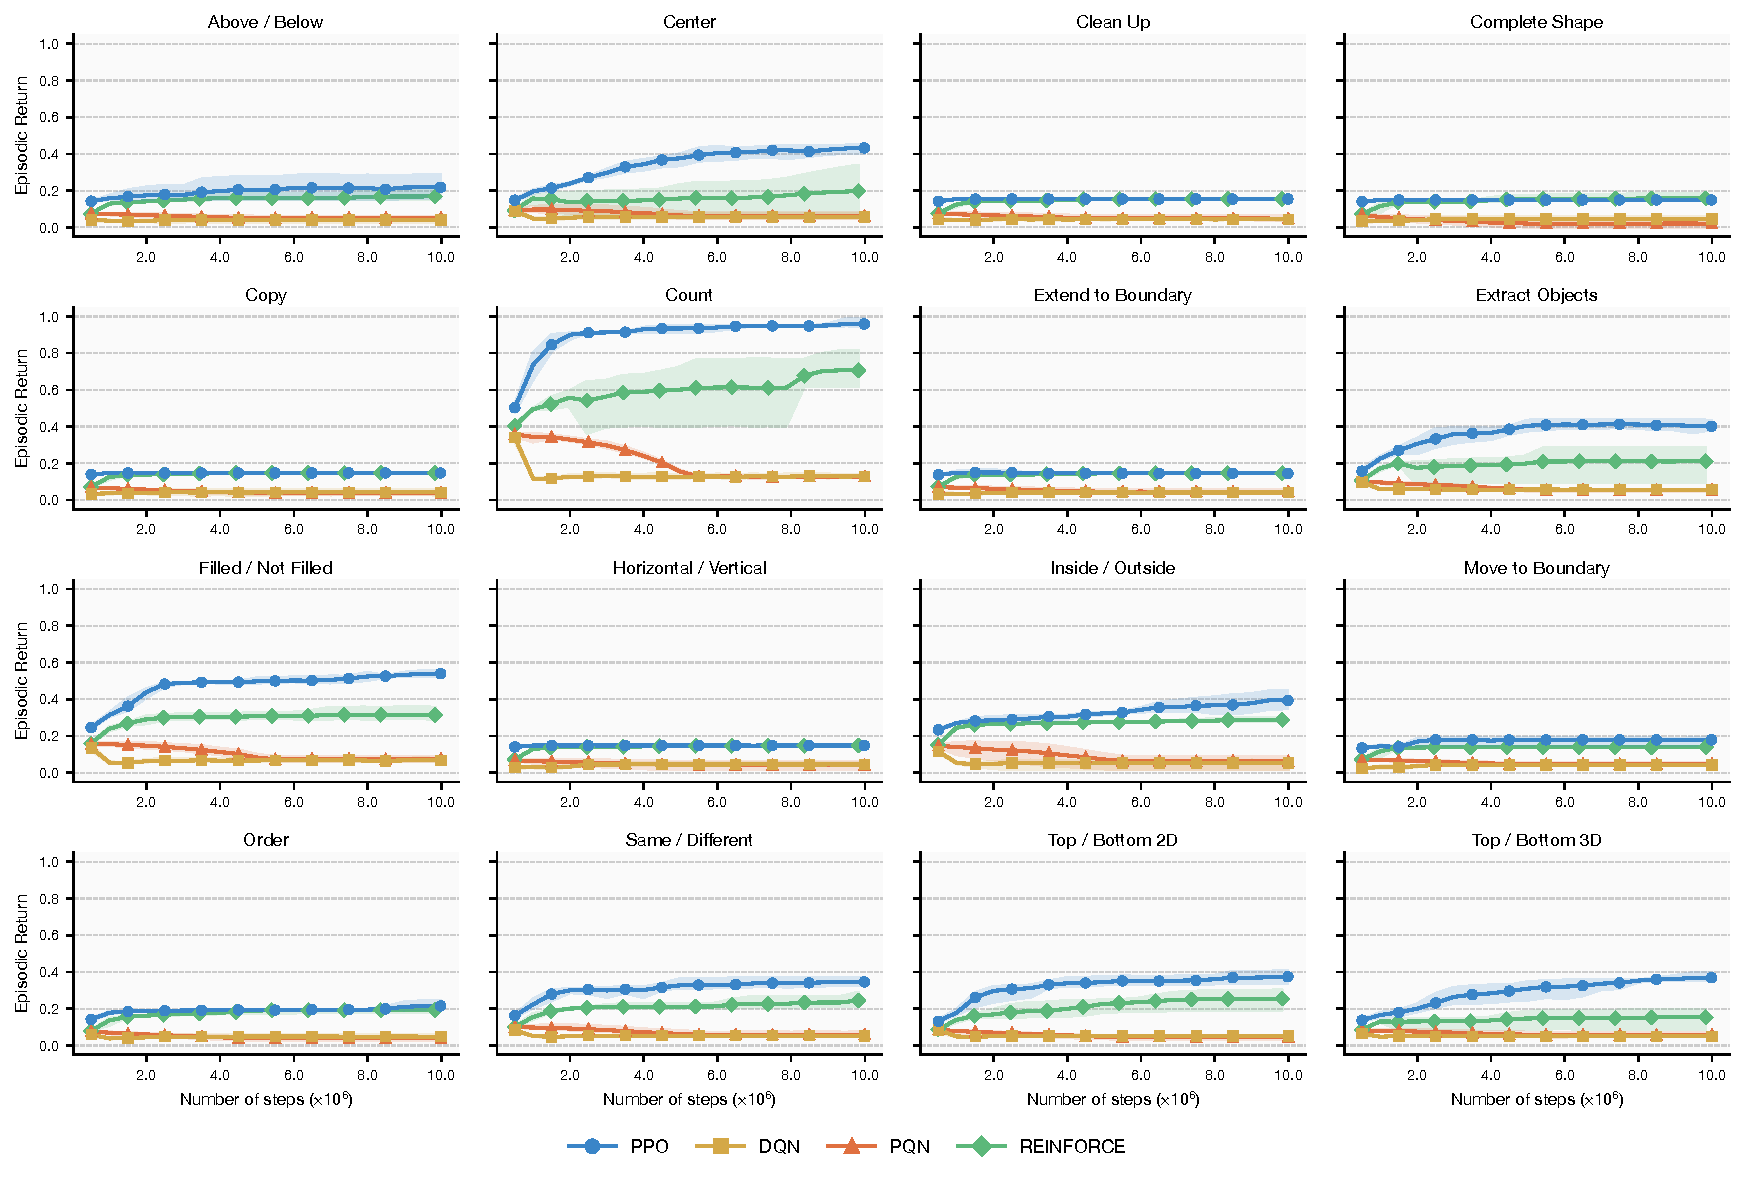
\includegraphics[width=0.95\linewidth]{Figures/conceptarc_episode_return.pdf}
\caption{Episodic return across all 16 ConceptARC concept groups.}
\label{fig:concept_episode_return_full}
\end{figure}

\begin{figure}[htbp]
\centering
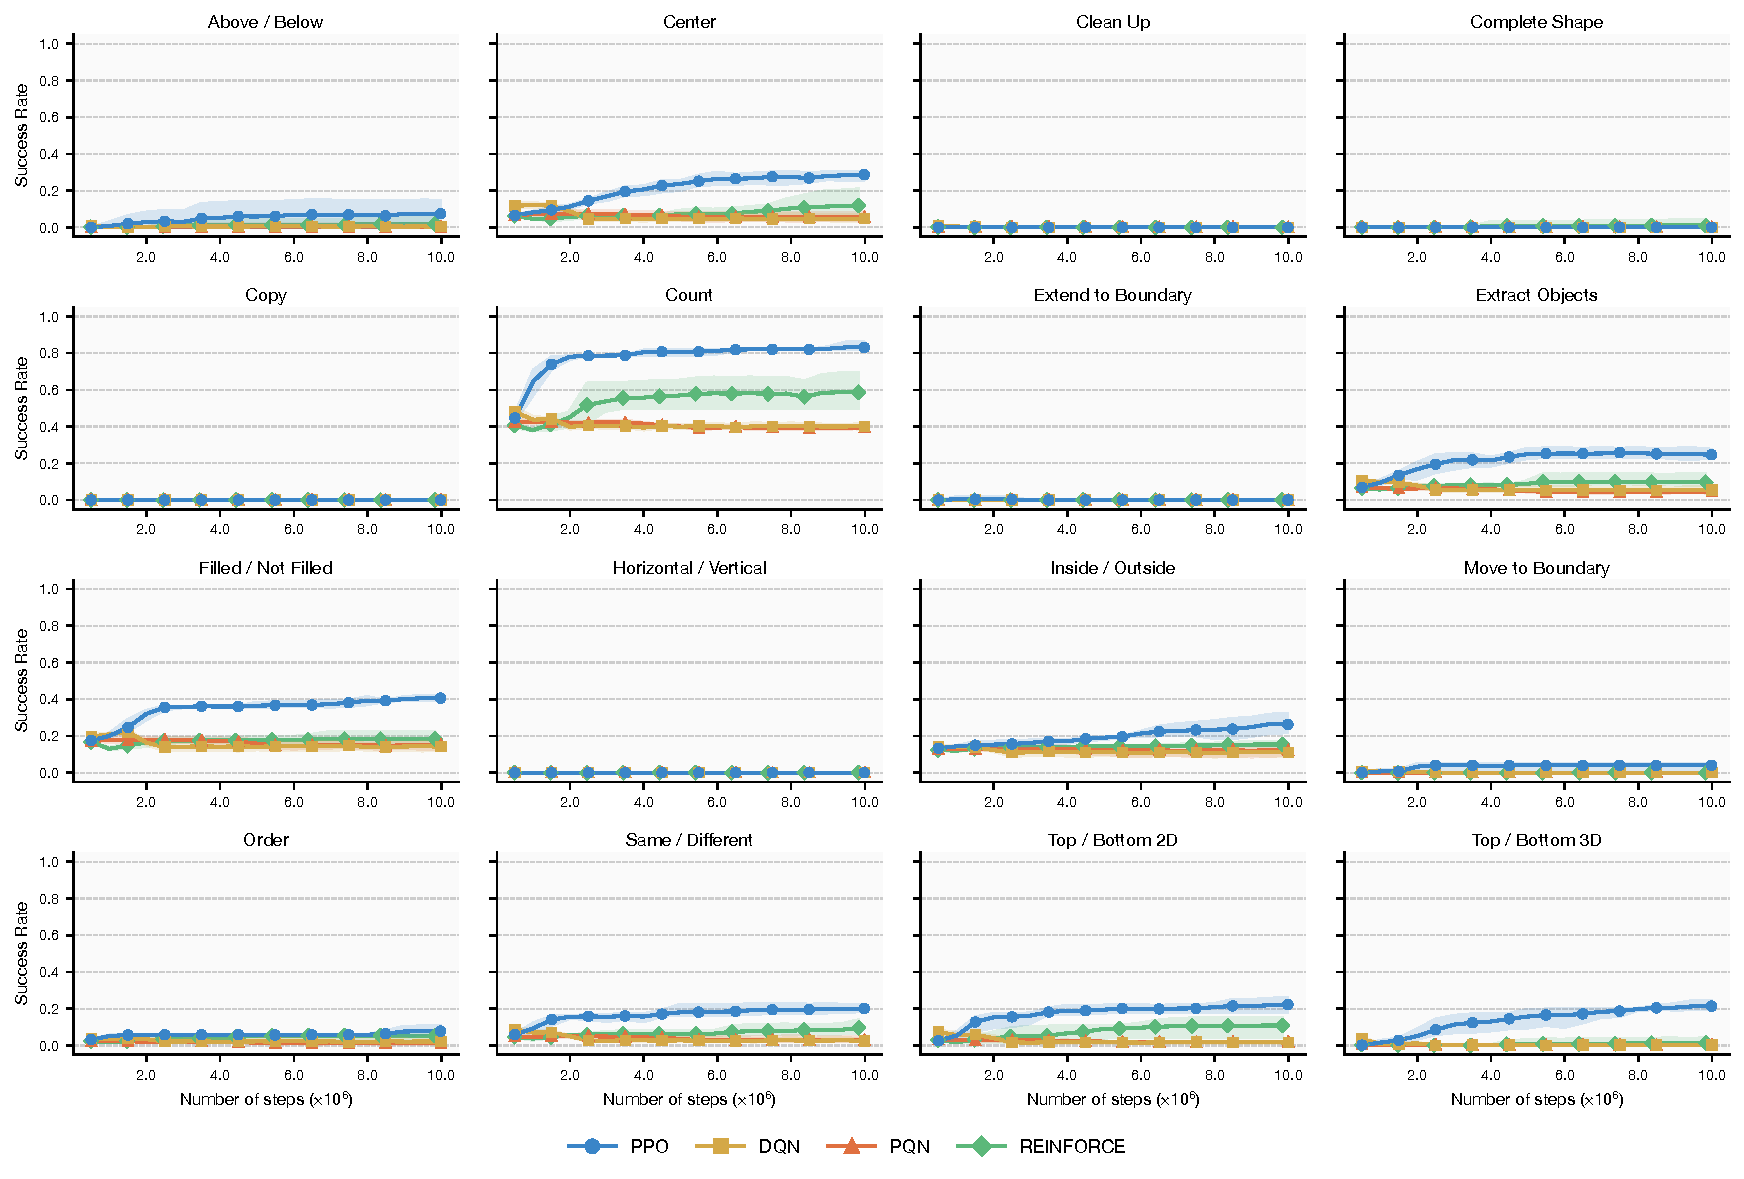
\includegraphics[width=0.95\linewidth]{Figures/conceptarc_success_rate.pdf}
\caption{Success rate across all 16 ConceptARC concept groups.}
\label{fig:concept_success_rate_full}
\end{figure}
\FloatBarrier


\newpage
\section*{NeurIPS Paper Checklist}

\begin{enumerate}

\item {\bf Claims}
    \item[] Question: Do the main claims made in the abstract and introduction accurately reflect the paper's contributions and scope?
    \item[] Answer: \answerYes{}.
    \item[] Justification: The abstract and introduction state the three contributions of this work: an accelerator-native ARC environment, a multi-algorithm RL baseline sweep over ARC-AGI-1 and ConceptARC, and an observation-wrapper diagnostic on MiniARC. They also report the same throughput numbers ($101.3$M SPS on a single H100, $790.4$M SPS with multi-device \texttt{pmap}, $5{,}439\times$ matched-batch speedup over ARCLE) presented in Section~\ref{sec:experiments} and Appendix~\ref{app:throughput}. 
    \item[] Guidelines:
    \begin{itemize}
        \item The answer \answerNA{} means that the abstract and introduction do not include the claims made in the paper.
        \item The abstract and/or introduction should clearly state the claims made, including the contributions made in the paper and important assumptions and limitations. A \answerNo{} or \answerNA{} answer to this question will not be perceived well by the reviewers. 
        \item The claims made should match theoretical and experimental results, and reflect how much the results can be expected to generalize to other settings. 
        \item It is fine to include aspirational goals as motivation as long as it is clear that these goals are not attained by the paper. 
    \end{itemize}

\item {\bf Limitations}
    \item[] Question: Does the paper discuss the limitations of the work performed by the authors?
    \item[] Answer: \answerYes{}.
    \item[] Justification: The Discussion contains a dedicated \emph{Limitations} paragraph stating that the baselines deliberately use a shallow two-layer CNN with $32$ channels, that the sweep covers only model-free training from scratch, and that meta-learning and test-time adaptation methods are not evaluated. The same paragraph clarifies that the reported curves should be read as fixed-interface lower bounds and not as upper bounds on what RL can achieve on ARC. The Discussion also notes that ARC-Game labels are subjective and that ARCLE crashes from memory exhaustion at large batch sizes, which bounds the matched comparison range.
    \item[] Guidelines:
    \begin{itemize}
        \item The answer \answerNA{} means that the paper has no limitation while the answer \answerNo{} means that the paper has limitations, but those are not discussed in the paper. 
        \item The authors are encouraged to create a separate ``Limitations'' section in their paper.
        \item The paper should point out any strong assumptions and how robust the results are to violations of these assumptions (e.g., independence assumptions, noiseless settings, model well-specification, asymptotic approximations only holding locally). The authors should reflect on how these assumptions might be violated in practice and what the implications would be.
        \item The authors should reflect on the scope of the claims made, e.g., if the approach was only tested on a few datasets or with a few runs. In general, empirical results often depend on implicit assumptions, which should be articulated.
        \item The authors should reflect on the factors that influence the performance of the approach. For example, a facial recognition algorithm may perform poorly when image resolution is low or images are taken in low lighting. Or a speech-to-text system might not be used reliably to provide closed captions for online lectures because it fails to handle technical jargon.
        \item The authors should discuss the computational efficiency of the proposed algorithms and how they scale with dataset size.
        \item If applicable, the authors should discuss possible limitations of their approach to address problems of privacy and fairness.
        \item While the authors might fear that complete honesty about limitations might be used by reviewers as grounds for rejection, a worse outcome might be that reviewers discover limitations that aren't acknowledged in the paper. The authors should use their best judgment and recognize that individual actions in favor of transparency play an important role in developing norms that preserve the integrity of the community. Reviewers will be specifically instructed to not penalize honesty concerning limitations.
    \end{itemize}

\item {\bf Theory assumptions and proofs}
    \item[] Question: For each theoretical result, does the paper provide the full set of assumptions and a complete (and correct) proof?
    \item[] Answer: \answerNA{}.
    \item[] Justification: The paper does not present theoretical results, theorems, or formal proofs.
    \item[] Guidelines:
    \begin{itemize}
        \item The answer \answerNA{} means that the paper does not include theoretical results. 
        \item All the theorems, formulas, and proofs in the paper should be numbered and cross-referenced.
        \item All assumptions should be clearly stated or referenced in the statement of any theorems.
        \item The proofs can either appear in the main paper or the supplemental material, but if they appear in the supplemental material, the authors are encouraged to provide a short proof sketch to provide intuition. 
        \item Inversely, any informal proof provided in the core of the paper should be complemented by formal proofs provided in appendix or supplemental material.
        \item Theorems and Lemmas that the proof relies upon should be properly referenced. 
    \end{itemize}

\item {\bf Experimental result reproducibility}
    \item[] Question: Does the paper fully disclose all the information needed to reproduce the main experimental results of the paper to the extent that it affects the main claims and/or conclusions of the paper (regardless of whether the code and data are provided or not)?
    \item[] Answer: \answerYes{}.
    \item[] Justification: Section~\ref{sec:experiments} states the throughput protocol, the per-condition training budget ($10^7$ environment steps), the seed count, the algorithms, and the hardware. Appendix~\ref{app:stoix} lists the common settings, the wrapper-chain order, and the per-algorithm hyperparameters. Appendix~\ref{app:throughput} states the exact ARCLE configuration used for matched comparison. Appendix~\ref{app:code_and_data} provides anonymized links to the JaxARC environment and the baselines code, including the Hydra configuration files used to launch every reported run.
    \item[] Guidelines:
    \begin{itemize}
        \item The answer \answerNA{} means that the paper does not include experiments.
        \item If the paper includes experiments, a \answerNo{} answer to this question will not be perceived well by the reviewers: Making the paper reproducible is important, regardless of whether the code and data are provided or not.
        \item If the contribution is a dataset and\slash or model, the authors should describe the steps taken to make their results reproducible or verifiable. 
        \item Depending on the contribution, reproducibility can be accomplished in various ways. For example, if the contribution is a novel architecture, describing the architecture fully might suffice, or if the contribution is a specific model and empirical evaluation, it may be necessary to either make it possible for others to replicate the model with the same dataset, or provide access to the model. In general. releasing code and data is often one good way to accomplish this, but reproducibility can also be provided via detailed instructions for how to replicate the results, access to a hosted model (e.g., in the case of a large language model), releasing of a model checkpoint, or other means that are appropriate to the research performed.
        \item While NeurIPS does not require releasing code, the conference does require all submissions to provide some reasonable avenue for reproducibility, which may depend on the nature of the contribution. For example
        \begin{enumerate}
            \item If the contribution is primarily a new algorithm, the paper should make it clear how to reproduce that algorithm.
            \item If the contribution is primarily a new model architecture, the paper should describe the architecture clearly and fully.
            \item If the contribution is a new model (e.g., a large language model), then there should either be a way to access this model for reproducing the results or a way to reproduce the model (e.g., with an open-source dataset or instructions for how to construct the dataset).
            \item We recognize that reproducibility may be tricky in some cases, in which case authors are welcome to describe the particular way they provide for reproducibility. In the case of closed-source models, it may be that access to the model is limited in some way (e.g., to registered users), but it should be possible for other researchers to have some path to reproducing or verifying the results.
        \end{enumerate}
    \end{itemize}


\item {\bf Open access to data and code}
    \item[] Question: Does the paper provide open access to the data and code, with sufficient instructions to faithfully reproduce the main experimental results, as described in supplemental material?
    \item[] Answer: \answerYes{}.
    \item[] Justification: Both code repositories are released as anonymized open-source projects for double-blind review (Appendix~\ref{app:code_and_data}): the JaxARC environment at \url{https://anonymous.4open.science/r/JaxARC-8788} and the baselines, configurations, and plotting scripts at \url{https://anonymous.4open.science/r/jaxarc-baselines-561F}. Both are MIT-licensed. Datasets used by the experiments (ARC-AGI-1, ARC-AGI-2, MiniARC, ConceptARC) are public and downloaded automatically by JaxARC's \texttt{auto\_download} hook from their upstream repositories.
    \item[] Guidelines:
    \begin{itemize}
        \item The answer \answerNA{} means that paper does not include experiments requiring code.
        \item Please see the NeurIPS code and data submission guidelines (\url{https://neurips.cc/public/guides/CodeSubmissionPolicy}) for more details.
        \item While we encourage the release of code and data, we understand that this might not be possible, so \answerNo{} is an acceptable answer. Papers cannot be rejected simply for not including code, unless this is central to the contribution (e.g., for a new open-source benchmark).
        \item The instructions should contain the exact command and environment needed to run to reproduce the results. See the NeurIPS code and data submission guidelines (\url{https://neurips.cc/public/guides/CodeSubmissionPolicy}) for more details.
        \item The authors should provide instructions on data access and preparation, including how to access the raw data, preprocessed data, intermediate data, and generated data, etc.
        \item The authors should provide scripts to reproduce all experimental results for the new proposed method and baselines. If only a subset of experiments are reproducible, they should state which ones are omitted from the script and why.
        \item At submission time, to preserve anonymity, the authors should release anonymized versions (if applicable).
        \item Providing as much information as possible in supplemental material (appended to the paper) is recommended, but including URLs to data and code is permitted.
    \end{itemize}


\item {\bf Experimental setting/details}
    \item[] Question: Does the paper specify all the training and test details (e.g., data splits, hyperparameters, how they were chosen, type of optimizer) necessary to understand the results?
    \item[] Answer: \answerYes{}.
    \item[] Justification: Section~\ref{sec:experiments} specifies the dataset splits, the per-run training budget, the number of seeds, the algorithm set, the metrics, the hardware platforms, and the rationale for the chosen interface. Appendix~\ref{app:stoix} provides the common settings (parallelization, episode limit, evaluation cadence, grid initializer), Appendix~\ref{app:baseline_hyperparameters} provides the per-algorithm hyperparameters, Appendix~\ref{app:network_architecture} provides the network architecture, and Appendix~\ref{app:reward_config} states the reward profile constants. Hyperparameters were selected for stable execution across many task families rather than per-task tuning, as discussed in Appendix~\ref{app:baseline_hyperparameters}.
    \item[] Guidelines:
    \begin{itemize}
        \item The answer \answerNA{} means that the paper does not include experiments.
        \item The experimental setting should be presented in the core of the paper to a level of detail that is necessary to appreciate the results and make sense of them.
        \item The full details can be provided either with the code, in appendix, or as supplemental material.
    \end{itemize}

\item {\bf Experiment statistical significance}
    \item[] Question: Does the paper report error bars suitably and correctly defined or other appropriate information about the statistical significance of the experiments?
    \item[] Answer: \answerYes{}.
    \item[] Justification: The throughput benchmark repeats each configuration $10$ times and reports the mean steady-state environment steps per second. Each baseline condition is trained with five independent random seeds; the episodic-return curves in Figure~\ref{fig:baseline_episode_return} and the extended figures in Appendix~\ref{app:extended_baselines} show the cross-seed mean as a solid line with $\pm 1$ standard deviation as the shaded region, computed pointwise across seeds.
    \item[] Guidelines:
    \begin{itemize}
        \item The answer \answerNA{} means that the paper does not include experiments.
        \item The authors should answer \answerYes{} if the results are accompanied by error bars, confidence intervals, or statistical significance tests, at least for the experiments that support the main claims of the paper.
        \item The factors of variability that the error bars are capturing should be clearly stated (for example, train/test split, initialization, random drawing of some parameter, or overall run with given experimental conditions).
        \item The method for calculating the error bars should be explained (closed form formula, call to a library function, bootstrap, etc.)
        \item The assumptions made should be given (e.g., Normally distributed errors).
        \item It should be clear whether the error bar is the standard deviation or the standard error of the mean.
        \item It is OK to report 1-sigma error bars, but one should state it. The authors should preferably report a 2-sigma error bar than state that they have a 96\% CI, if the hypothesis of Normality of errors is not verified.
        \item For asymmetric distributions, the authors should be careful not to show in tables or figures symmetric error bars that would yield results that are out of range (e.g., negative error rates).
        \item If error bars are reported in tables or plots, the authors should explain in the text how they were calculated and reference the corresponding figures or tables in the text.
    \end{itemize}

\item {\bf Experiments compute resources}
    \item[] Question: For each experiment, does the paper provide sufficient information on the computer resources (type of compute workers, memory, time of execution) needed to reproduce the experiments?
    \item[] Answer: \answerYes{}.
    \item[] Justification: Section~\ref{sec:experiments} and Appendix~\ref{app:throughput} list the three hardware platforms used for the throughput benchmark (Apple M2 Pro CPU, NVIDIA RTX 3090 with $24$\,GB, NVIDIA H100 with $80$\,GB). Appendix~\ref{app:compute_env} states that each baseline run used a single H100 with $512$ vectorized environments and a $10^7$-step budget, taking on the order of one to two hours of wall-clock time per run, for a total sweep of $700$ runs ($4$ algorithms $\times$ $35$ subsets $\times$ $5$ seeds, $7\times 10^9$ environment steps). The same appendix lists the pinned software environment used for the throughput measurements (Python 3.13.5, JAX 0.6.2, NumPy 2.3.1, Gymnasium 1.2.0).
    \item[] Guidelines:
    \begin{itemize}
        \item The answer \answerNA{} means that the paper does not include experiments.
        \item The paper should indicate the type of compute workers CPU or GPU, internal cluster, or cloud provider, including relevant memory and storage.
        \item The paper should provide the amount of compute required for each of the individual experimental runs as well as estimate the total compute. 
        \item The paper should disclose whether the full research project required more compute than the experiments reported in the paper (e.g., preliminary or failed experiments that didn't make it into the paper). 
    \end{itemize}
    
\item {\bf Code of ethics}
    \item[] Question: Does the research conducted in the paper conform, in every respect, with the NeurIPS Code of Ethics \url{https://neurips.cc/public/EthicsGuidelines}?
    \item[] Answer: \answerYes{}.
    \item[] Justification: The work uses public, openly licensed benchmark datasets and reports infrastructure and baseline experiments. It does not involve human subjects, private data, or deployment of any model in a high-risk setting.
    \item[] Guidelines:
    \begin{itemize}
        \item The answer \answerNA{} means that the authors have not reviewed the NeurIPS Code of Ethics.
        \item If the authors answer \answerNo, they should explain the special circumstances that require a deviation from the Code of Ethics.
        \item The authors should make sure to preserve anonymity (e.g., if there is a special consideration due to laws or regulations in their jurisdiction).
    \end{itemize}


\item {\bf Broader impacts}
    \item[] Question: Does the paper discuss both potential positive societal impacts and negative societal impacts of the work performed?
    \item[] Answer: \answerYes{}.
    \item[] Justification: The Discussion contains a \emph{Broader Impact and Sustainability} paragraph noting that lowering the compute requirements of large-scale ARC RL experiments broadens access to teams without dedicated CPU clusters and reduces the energy spent per rollout for the same scientific question. The work releases an environment and reproducible baselines rather than a deployed decision system or a high-capability generative model, so the direct path to negative downstream applications is limited.
    \item[] Guidelines:
    \begin{itemize}
        \item The answer \answerNA{} means that there is no societal impact of the work performed.
        \item If the authors answer \answerNA{} or \answerNo, they should explain why their work has no societal impact or why the paper does not address societal impact.
        \item Examples of negative societal impacts include potential malicious or unintended uses (e.g., disinformation, generating fake profiles, surveillance), fairness considerations (e.g., deployment of technologies that could make decisions that unfairly impact specific groups), privacy considerations, and security considerations.
        \item The conference expects that many papers will be foundational research and not tied to particular applications, let alone deployments. However, if there is a direct path to any negative applications, the authors should point it out. For example, it is legitimate to point out that an improvement in the quality of generative models could be used to generate Deepfakes for disinformation. On the other hand, it is not needed to point out that a generic algorithm for optimizing neural networks could enable people to train models that generate Deepfakes faster.
        \item The authors should consider possible harms that could arise when the technology is being used as intended and functioning correctly, harms that could arise when the technology is being used as intended but gives incorrect results, and harms following from (intentional or unintentional) misuse of the technology.
        \item If there are negative societal impacts, the authors could also discuss possible mitigation strategies (e.g., gated release of models, providing defenses in addition to attacks, mechanisms for monitoring misuse, mechanisms to monitor how a system learns from feedback over time, improving the efficiency and accessibility of ML).
    \end{itemize}
    
\item {\bf Safeguards}
    \item[] Question: Does the paper describe safeguards that have been put in place for responsible release of data or models that have a high risk for misuse (e.g., pre-trained language models, image generators, or scraped datasets)?
    \item[] Answer: \answerNA{}.
    \item[] Justification: The released artifact is a deterministic simulator for an existing public benchmark and a set of small RL training scripts.
    \item[] Guidelines:
    \begin{itemize}
        \item The answer \answerNA{} means that the paper poses no such risks.
        \item Released models that have a high risk for misuse or dual-use should be released with necessary safeguards to allow for controlled use of the model, for example by requiring that users adhere to usage guidelines or restrictions to access the model or implementing safety filters. 
        \item Datasets that have been scraped from the Internet could pose safety risks. The authors should describe how they avoided releasing unsafe images.
        \item We recognize that providing effective safeguards is challenging, and many papers do not require this, but we encourage authors to take this into account and make a best faith effort.
    \end{itemize}

\item {\bf Licenses for existing assets}
    \item[] Question: Are the creators or original owners of assets (e.g., code, data, models), used in the paper, properly credited and are the license and terms of use explicitly mentioned and properly respected?
    \item[] Answer: \answerYes{}.
    \item[] Justification: All datasets, software libraries, and prior environments used in the paper are cited at first use. The four ARC datasets are public and openly licensed: ARC-AGI-1 \citep{cholletMeasureIntelligence2019}, ARC-AGI-2 \citep{cholletARCAGI2NewChallenge2025}, and MiniARC \citep{kimPlaygroundsAbstractionReasoning2022} are distributed under the Apache 2.0 license; ConceptARC \citep{moskvichevConceptARCBenchmarkEvaluating2023} is distributed under the MIT license. The supporting libraries are similarly attributed: ARCLE \citep{leeARCLEAbstractionReasonin2024} for the comparison baseline, and Stoix \citep{toledoStoixDistributedSingleagent2024} together with Stoa \citep{toledoStoaJAXnativeInterface2025} for the training framework and environment interface. Local snapshots of every dataset retain their upstream \texttt{LICENSE} files (Appendix~\ref{app:code_and_data}), and JaxARC's downloader fetches each dataset from its official upstream repository so that license terms are respected at runtime.
    \item[] Guidelines:
    \begin{itemize}
        \item The answer \answerNA{} means that the paper does not use existing assets.
        \item The authors should cite the original paper that produced the code package or dataset.
        \item The authors should state which version of the asset is used and, if possible, include a URL.
        \item The name of the license (e.g., CC-BY 4.0) should be included for each asset.
        \item For scraped data from a particular source (e.g., website), the copyright and terms of service of that source should be provided.
        \item If assets are released, the license, copyright information, and terms of use in the package should be provided. For popular datasets, \url{paperswithcode.com/datasets} has curated licenses for some datasets. Their licensing guide can help determine the license of a dataset.
        \item For existing datasets that are re-packaged, both the original license and the license of the derived asset (if it has changed) should be provided.
        \item If this information is not available online, the authors are encouraged to reach out to the asset's creators.
    \end{itemize}

\item {\bf New assets}
    \item[] Question: Are new assets introduced in the paper well documented and is the documentation provided alongside the assets?
    \item[] Answer: \answerYes{}.
    \item[] Justification: JaxARC and the baselines code are the new software assets introduced by this paper. Both are released under the MIT license at the anonymized URLs in Appendix~\ref{app:code_and_data}. The manuscript documents the environment API (Appendix~\ref{app:usage}), the internal data structures (Appendix~\ref{app:data_structures}), the reset and step semantics (Appendix~\ref{app:reset_and_step}), the similarity score (Appendix~\ref{app:similarity}), the working-grid initialization strategies (Appendix~\ref{app:grid_init}), the action and observation wrappers (Appendices~\ref{app:action_config} and~\ref{app:observation_wrappers}), the reward profiles (Appendix~\ref{app:reward_config}), the dataset registration interface (Appendix~\ref{app:extensibility}), the wrapper chain used by the baselines (Appendix~\ref{app:stoix}), and the per-algorithm hyperparameters and architecture (Appendices~\ref{app:baseline_hyperparameters} and~\ref{app:network_architecture}). The repositories include README files, example scripts, and the Hydra configurations needed to reproduce every reported experiment.
    \item[] Guidelines:
    \begin{itemize}
        \item The answer \answerNA{} means that the paper does not release new assets.
        \item Researchers should communicate the details of the dataset\slash code\slash model as part of their submissions via structured templates. This includes details about training, license, limitations, etc. 
        \item The paper should discuss whether and how consent was obtained from people whose asset is used.
        \item At submission time, remember to anonymize your assets (if applicable). You can either create an anonymized URL or include an anonymized zip file.
    \end{itemize}

\item {\bf Crowdsourcing and research with human subjects}
    \item[] Question: For crowdsourcing experiments and research with human subjects, does the paper include the full text of instructions given to participants and screenshots, if applicable, as well as details about compensation (if any)? 
    \item[] Answer: \answerNA{}.
    \item[] Justification: The paper does not involve crowdsourcing or new research with human subjects. All datasets used in the experiments are pre-existing public benchmarks; the paper does not collect any new human data.
    \item[] Guidelines:
    \begin{itemize}
        \item The answer \answerNA{} means that the paper does not involve crowdsourcing nor research with human subjects.
        \item Including this information in the supplemental material is fine, but if the main contribution of the paper involves human subjects, then as much detail as possible should be included in the main paper. 
        \item According to the NeurIPS Code of Ethics, workers involved in data collection, curation, or other labor should be paid at least the minimum wage in the country of the data collector. 
    \end{itemize}

\item {\bf Institutional review board (IRB) approvals or equivalent for research with human subjects}
    \item[] Question: Does the paper describe potential risks incurred by study participants, whether such risks were disclosed to the subjects, and whether Institutional Review Board (IRB) approvals (or an equivalent approval/review based on the requirements of your country or institution) were obtained?
    \item[] Answer: \answerNA{}.
    \item[] Justification: The paper does not involve human subjects.
    \item[] Guidelines:
    \begin{itemize}
        \item The answer \answerNA{} means that the paper does not involve crowdsourcing nor research with human subjects.
        \item Depending on the country in which research is conducted, IRB approval (or equivalent) may be required for any human subjects research. If you obtained IRB approval, you should clearly state this in the paper. 
        \item We recognize that the procedures for this may vary significantly between institutions and locations, and we expect authors to adhere to the NeurIPS Code of Ethics and the guidelines for their institution. 
        \item For initial submissions, do not include any information that would break anonymity (if applicable), such as the institution conducting the review.
    \end{itemize}

\item {\bf Declaration of LLM usage}
    \item[] Question: Does the paper describe the usage of LLMs if it is an important, original, or non-standard component of the core methods in this research? Note that if the LLM is used only for writing, editing, or formatting purposes and does \emph{not} impact the core methodology, scientific rigor, or originality of the research, declaration is not required.
    %this research? 
    \item[] Answer: \answerNA{}.
    \item[] Justification: LLMs are not part of the core method/environment.
    \item[] Guidelines:
    \begin{itemize}
        \item The answer \answerNA{} means that the core method development in this research does not involve LLMs as any important, original, or non-standard components.
        \item Please refer to our LLM policy in the NeurIPS handbook for what should or should not be described.
    \end{itemize}

\end{enumerate}


\end{document}